% ============================================================================
% OFFCUTS -- material removed from main.tex during the shortening pass.
%
% This document is NOT part of the thesis. It is never \input into main.tex and
% it is excluded from the submitted archive. It exists so that every removal is
% a MOVE rather than a deletion: each excerpt below is the live source, rendered
% with the thesis's own preamble, so it looks the way it looked in the thesis
% and can be pasted straight back.
%
% Baseline: everything here was cut from commit d4d5a0d.
% Build:    latexmk -pdf offcuts.tex   (after main.tex has been built once, so
%           main.aux exists for xr to read).
% ============================================================================

% ============================================================================
% COMPREHENSIVE PREAMBLE FOR ERDOS PROBLEM 915 THESIS
% ============================================================================

\documentclass[kul, 11pt, a4paper, oneside]{kulakreport}
\usetikzlibrary{calc, arrows.meta, shapes.geometric, decorations.markings}

% KU Leuven metadata
\faculty{Faculty of Science}
\group{Department of Mathematics}
\subtitle{Erd\H{o}s Problem 915, from Proof to Search}
\institute{Master of Mathematics}
\emailaddress{louis.vandenbruwaene@student.kuleuven.be}
\address{
   \textbf{KU Leuven} \\
   \textbf{Faculty of Science} \\
   Celestijnenlaan 200B, 3001 Leuven \\
   Belgium
}

% ============================================================================
% BASIC PACKAGES
% ============================================================================
\usepackage[utf8]{inputenc}
\usepackage[T1]{fontenc}
\usepackage[scaled=0.95]{helvet}
\renewcommand{\familydefault}{\sfdefault}
\usepackage[absolute,overlay]{textpos}
% lmodern not available; disable microtype expansion to avoid font errors
\usepackage[patch=none, expansion=false]{microtype}

% ============================================================================
% PAGE LAYOUT
% ============================================================================
\usepackage[
    a4paper,
    inner=25mm,
    outer=25mm,
    top=30mm,
    bottom=30mm,
    bindingoffset=5mm
]{geometry}

\usepackage{setspace}
\onehalfspacing

% Improve line breaking to reduce overfull hbox warnings
\tolerance=1414
\emergencystretch=1.5em
\hfuzz=3pt
\vfuzz=3pt

% ============================================================================
% MATHEMATICS
% ============================================================================
\usepackage{amsmath, amssymb, amsthm}
\usepackage{mathtools}
\usepackage{bm}

% ============================================================================
% GRAPHICS AND COLOR (tikz, graphicx, xcolor already loaded by kulakreport)
% ============================================================================
\usetikzlibrary{positioning, arrows.meta, calc, shapes.geometric,
                decorations.pathmorphing, backgrounds, fit,
                patterns, shadows, matrix}

% ============================================================================
% FIGURES AND TABLES
% ============================================================================
\usepackage{float}
% rotating: the twelve-panel bounds grid needs a full sideways page, since at
% text width its per-panel labels fall under 2pt.
\usepackage{rotating}
\usepackage{caption}
\usepackage{subcaption}
\usepackage{booktabs}
\usepackage{array}
\usepackage{multirow}

% Uniform caption look for every plot, figure, and table: a bold blue label, a
% slightly smaller justified body set in from the margins, and a touch of space
% above so a caption never crowds the artwork it describes.
\captionsetup{
    font=small,
    labelfont={bf,color=KULblauw3b},
    textfont={color=black!85},
    labelsep=period,
    justification=justified,
    singlelinecheck=true,
    margin=14pt,
    skip=8pt,
}
\captionsetup[sub]{
    font=footnotesize,
    labelfont={bf,color=KULblauw3b},
    % Ragged right, not justified: sub-captions often sit in narrow boxes
    % (half-width panels), where justification stretches short lines into
    % wide word gaps around unbreakable math.
    justification=raggedright,
    margin=4pt,
    skip=5pt,
}

% ============================================================================
% LISTS
% ============================================================================
\usepackage{enumitem}

% Custom bullet styles using small graph icons
\newcommand{\prettygrotzsch}{%
	\tikz[baseline=-0.6ex, scale=0.12]{
		\definecolor{nodecolor}{RGB}{50, 120, 180}
		\foreach \i in {0,...,4} {
			\coordinate (inner\i) at ({1.2*cos(72*\i+18)},{1.2*sin(72*\i+18)});
		}
		\coordinate (center) at (0,0);
		\draw[nodecolor, line width=0.5pt]
		(center) -- (inner0) (center) -- (inner1) (center) -- (inner2)
		(center) -- (inner3) (center) -- (inner4)
		(inner0) -- (inner2) (inner0) -- (inner3) (inner1) -- (inner3)
		(inner1) -- (inner4) (inner2) -- (inner4);
		\foreach \i in {0,...,4} { \fill[black] (inner\i) circle (2.5pt); }
		\fill[black] (center) circle (2.5pt);
	}
}

\newcommand{\prettypetersen}{%
	\tikz[baseline=-0.6ex, scale=0.15]{
		\definecolor{petersennode}{RGB}{20, 140, 140}
		\definecolor{petersenedge}{RGB}{100, 100, 100}

		\def\R{1.2}
		\def\r{0.8}

		\foreach \i in {0,...,4} {
			\coordinate (outer\i) at ({90+72*\i}:\R);
			\coordinate (inner\i) at ({90+72*\i}:\r);
		}

		\foreach \i in {0,...,4} {
			\fill[petersennode] (outer\i) circle (4pt);
			\fill[petersennode] (inner\i) circle (4pt);
		}

		\draw[petersenedge, line width=0.7pt]
		(outer0) -- (outer1) -- (outer2) -- (outer3) -- (outer4) -- (outer0)
		(outer0) -- (inner0)
		(outer1) -- (inner1)
		(outer2) -- (inner2)
		(outer3) -- (inner3)
		(outer4) -- (inner4)
		(inner0) -- (inner2) -- (inner4) -- (inner1) -- (inner3) -- (inner0);

		\foreach \i in {0,...,4} {
			\fill[black, opacity=1] (outer\i) circle (3pt);
			\fill[black, opacity=1] (inner\i) circle (3pt);
		}
	}
}

\setlist[itemize]{label=$\prettygrotzsch$, leftmargin=1.5em}
\setlist[enumerate]{label=\protect\prettypetersen, leftmargin=2em}

% ============================================================================
% HYPERLINKS AND REFERENCES
% ============================================================================
\usepackage[noabbrev, capitalize, nameinlink]{cleveref}

% ============================================================================
% BIBLIOGRAPHY
% ============================================================================
\usepackage[numbers, sort&compress]{natbib}

% ============================================================================
% HEADER/FOOTER
% ============================================================================
% The page footer ("section mark | page number") is defined by the kulakreport
% class with oneside-friendly specifiers; nothing to add here.

% ============================================================================
% CHAPTER STYLING
% ============================================================================
\usepackage{titlesec}
% Chapter: keep the large black title, but brand the "Chapter N" label in the
% KU Leuven house blue so the heading reads as part of the institutional style.
\titleformat{\chapter}[display]
  {\normalfont\huge\bfseries}{\color{KULblauw1}\chaptertitlename\ \thechapter}{20pt}{\Huge\raggedright}
\titlespacing*{\chapter}{0pt}{-30pt}{40pt}

% Section headings: black bold title with a blue section number and a thin blue
% accent rule beneath, matching the chapter branding and easing navigation in
% the long chapters. Subsection and below stay quieter, with only a blue number.
\titleformat{\section}
  {\normalfont\Large\bfseries}{\color{KULblauw1}\thesection}{0.7em}{}
\titlespacing*{\section}{0pt}{1.8ex plus .3ex minus .2ex}{0.9ex}

\titleformat{\subsection}
  {\normalfont\large\bfseries}{\color{KULblauw1}\thesubsection}{0.6em}{}
\titlespacing*{\subsection}{0pt}{1.4ex plus .2ex minus .2ex}{0.6ex}

\titleformat{\subsubsection}
  {\normalfont\normalsize\bfseries}{\color{KULblauw1}\thesubsubsection}{0.5em}{}
\titlespacing*{\subsubsection}{0pt}{1.1ex plus .2ex minus .2ex}{0.5ex}

\titleformat{\paragraph}[runin]
  {\normalfont\normalsize\bfseries\color{KULblauw3b}}{}{0pt}{}
\titlespacing*{\paragraph}{0pt}{1ex plus .2ex minus .1ex}{0.8em}

% Part openers carry a framing paragraph rather than sitting as an empty page.
% The "top" class starts a new page with the banner at the top, then lets the
% following text flow on the same page.
\titleclass{\part}{top}
\titleformat{\part}[display]
  {\normalfont\Huge\bfseries\color{KULblauw3b}}{\partname\ \thepart}{0.4em}{\Huge}
\titlespacing*{\part}{0pt}{0pt}{1.5em}

% ============================================================================
% THEOREM ENVIRONMENTS (using aliascnt for proper cleveref support)
% ============================================================================
\usepackage{aliascnt}

% Base theorem
\theoremstyle{plain}
\newtheorem{theorem}{Theorem}[chapter]

% Theorem-like (italic body) - with aliascnt for cleveref
\newaliascnt{proposition}{theorem}
\newtheorem{proposition}[proposition]{Proposition}
\aliascntresetthe{proposition}

\newaliascnt{lemma}{theorem}
\newtheorem{lemma}[lemma]{Lemma}
\aliascntresetthe{lemma}

\newaliascnt{corollary}{theorem}
\newtheorem{corollary}[corollary]{Corollary}
\aliascntresetthe{corollary}

\newaliascnt{conjecture}{theorem}
\newtheorem{conjecture}[conjecture]{Conjecture}
\aliascntresetthe{conjecture}

\newaliascnt{claim}{theorem}
\newtheorem{claim}[claim]{Claim}
\aliascntresetthe{claim}

% Definition-like (upright body)
\theoremstyle{definition}
\newaliascnt{definition}{theorem}
\newtheorem{definition}[definition]{Definition}
\aliascntresetthe{definition}

\newaliascnt{example}{theorem}
\newtheorem{example}[example]{Example}
\aliascntresetthe{example}

\newaliascnt{construction}{theorem}
\newtheorem{construction}[construction]{Construction}
\aliascntresetthe{construction}

% Remark-like
\theoremstyle{remark}
\newaliascnt{remark}{theorem}
\newtheorem{remark}[remark]{Remark}
\aliascntresetthe{remark}

\newaliascnt{notation}{theorem}
\newtheorem{notation}[notation]{Notation}
\aliascntresetthe{notation}

\newaliascnt{ques}{theorem}
\newtheorem{ques}[ques]{Question}
\aliascntresetthe{ques}

% Unnumbered versions
\newtheorem*{theorem*}{Theorem}
\newtheorem*{remark*}{Remark}

% Custom proof environment for claims
\newenvironment{claimproof}[1][\proofname]{\begin{proof}[#1]\renewcommand{\qedsymbol}{$\diamondsuit$}}{\end{proof}}

% Cleveref settings (must be after theorem environment definitions)
\crefname{theorem}{theorem}{theorems}
\Crefname{theorem}{Theorem}{Theorems}
\crefname{proposition}{proposition}{propositions}
\Crefname{proposition}{Proposition}{Propositions}
\crefname{lemma}{lemma}{lemmas}
\Crefname{lemma}{Lemma}{Lemmas}
\crefname{corollary}{corollary}{corollaries}
\Crefname{corollary}{Corollary}{Corollaries}
\crefname{conjecture}{conjecture}{conjectures}
\Crefname{conjecture}{Conjecture}{Conjectures}
\crefname{definition}{definition}{definitions}
\Crefname{definition}{Definition}{Definitions}
\crefname{example}{example}{examples}
\Crefname{example}{Example}{Examples}
\crefname{remark}{remark}{remarks}
\Crefname{remark}{Remark}{Remarks}
\crefname{construction}{construction}{constructions}
\Crefname{construction}{Construction}{Constructions}
\crefname{ques}{question}{questions}
\Crefname{ques}{Question}{Questions}
\crefname{chapter}{Chapter}{Chapters}
\crefname{appendix}{Appendix}{Appendices}
\Crefname{appendix}{Appendix}{Appendices}
\crefname{section}{Section}{Sections}
\crefname{part}{Part}{Parts}
\crefname{figure}{Figure}{Figures}
\crefname{table}{Table}{Tables}

% ============================================================================
% CUSTOM MATHEMATICAL COMMANDS
% ============================================================================

% Floor and ceiling
\newcommand*{\floor}[1]{\left\lfloor #1 \right\rfloor}
\newcommand*{\ceil}[1]{\left\lceil #1 \right\rceil}
\newcommand*{\floorfrac}[2]{\floor{\frac{#1}{#2}}}
\newcommand*{\ceilfrac}[2]{\ceil{\frac{#1}{#2}}}

% Absolute value and norms
\newcommand*{\abs}[1]{\left\lvert #1 \right\rvert}
\newcommand*{\norm}[1]{\left\lVert #1 \right\rVert}

% Graph theory notation
\newcommand{\lec}{\lambda}                    % Local edge-connectivity
\newcommand{\kap}{\kappa}                     % Local vertex-connectivity
\newcommand{\multigraph}{\mathcal{M}}         % Multigraph
\newcommand{\HH}{\mathcal{H}}                 % Hypergraph
\DeclareMathOperator{\dist}{dist}             % Distance

% Probability notation
\DeclareMathOperator{\Var}{Var}               % Variance

% Common sets
\newcommand{\N}{\mathbb{N}}
\newcommand{\Z}{\mathbb{Z}}
\newcommand{\R}{\mathbb{R}}

% ============================================================================
% TIKZ STYLES - Unified Colors and Styles (from shared/)
% ============================================================================

% Import shared color definitions and TikZ styles
% ============================================================================
% UNIFIED COLOR DEFINITIONS FOR ERDOS PROBLEM 915 THESIS
% ============================================================================
% This file provides consistent colors across thesis, progress report, and
% presentation. All colors are based on KU Leuven institutional branding.
% ============================================================================

% --- KU Leuven Primary Colors ---
% Note: In beamer (kulakbeamer), KULblauw1/KULblauw3a/KULblauw3b are predefined
% For thesis documents, we define them here
\makeatletter
\@ifclassloaded{kulakbeamer}{%
    % Colors already defined by beamer class
}{%
    % Define KUL colors for non-beamer documents
    \definecolor{KULblauw1}{RGB}{29,141,176}     % Main blue
    \definecolor{KULblauw3a}{RGB}{82,189,236}    % Accent light blue
    \definecolor{KULblauw3b}{RGB}{30,110,135}    % Accent dark blue
}
\makeatother

% --- Graph Vertex Colors ---
% Primary vertex color uses KUL blue
\definecolor{vertexblue}{RGB}{29,141,176}        % KULblauw1
\definecolor{vertexred}{RGB}{200,80,80}          % Matched with presentation
\definecolor{vertexpurple}{RGB}{140,80,160}      % Matched with presentation
\definecolor{vertexgreen}{RGB}{60,160,80}        % Matched with presentation
\definecolor{vertexorange}{RGB}{220,140,40}      % Matched with presentation

% --- Aliases for presentation compatibility ---
\colorlet{graphred}{vertexred}
\colorlet{graphpurple}{vertexpurple}
\colorlet{graphgreen}{vertexgreen}
\colorlet{graphorange}{vertexorange}

% ============================================================================
% UNIFIED TIKZ STYLES FOR ERDOS PROBLEM 915 THESIS
% ============================================================================
% This file provides consistent TikZ graph styles across thesis, progress
% report, and presentation. Requires colors.tex to be loaded first.
% ============================================================================

% --- Vertex Styles ---
\tikzset{
    % Basic vertex style (KUL blue)
    vertex/.style={
        circle, draw=KULblauw1, fill=KULblauw1!15,
        minimum size=20pt, inner sep=0pt,
        font=\small\bfseries, line width=1.5pt
    },
    % Small vertex for complex diagrams
    smallvertex/.style={
        circle, draw=KULblauw1, fill=KULblauw1!15,
        minimum size=16pt, inner sep=0pt,
        font=\scriptsize\bfseries, line width=1.2pt
    },
    % Colored variants - semantic naming
    leftvertex/.style={vertex, draw=KULblauw1, fill=KULblauw1!15},
    rightvertex/.style={vertex, draw=vertexred, fill=vertexred!15},
    sharedvertex/.style={vertex, draw=vertexpurple, fill=vertexpurple!20},
    tailvertex/.style={vertex, draw=vertexgreen, fill=vertexgreen!15},
    hubvertex/.style={vertex, draw=vertexorange, fill=vertexorange!20},
    % Small colored variants
    smallleftvertex/.style={smallvertex, draw=KULblauw1, fill=KULblauw1!15},
    smallrightvertex/.style={smallvertex, draw=vertexred, fill=vertexred!15},
    smallsharedvertex/.style={smallvertex, draw=vertexpurple, fill=vertexpurple!20},
    smalltailvertex/.style={smallvertex, draw=vertexgreen, fill=vertexgreen!15},
    % Presentation-style aliases (gnode = graph node)
    gnode/.style={vertex},
    bluenode/.style={leftvertex},
    rednode/.style={rightvertex},
    purplenode/.style={sharedvertex},
    greennode/.style={tailvertex},
    orangenode/.style={hubvertex},
}

% --- Edge Styles ---
\tikzset{
    % Basic edge styles
    edge/.style={line width=1.8pt, KULblauw1!70},
    thickedge/.style={line width=2.5pt},
    % Colored edge variants - semantic naming
    leftedge/.style={line width=1.8pt, KULblauw1},
    rightedge/.style={line width=1.8pt, vertexred},
    sharededge/.style={line width=1.8pt, vertexpurple!80},
    tailedge/.style={line width=1.8pt, vertexgreen!80!black},
    % Tree edges
    treeedge/.style={line width=1.8pt, KULblauw3b},
    lefttreeedge/.style={line width=1.8pt, KULblauw1},
    righttreeedge/.style={line width=1.8pt, vertexred},
    % Special edge styles
    missingedge/.style={line width=1.5pt, dashed, gray},
    multiedge/.style={line width=1.5pt, draw=KULblauw3b},
    hyperedge/.style={draw=vertexred, fill=vertexred!10, rounded corners=8pt, line width=1.5pt},
    % Presentation-style aliases
    gedge/.style={line width=2pt, KULblauw1!70},
    blueedge/.style={line width=2pt, KULblauw1},
    rededge/.style={line width=2pt, vertexred},
    purpleedge/.style={line width=2pt, vertexpurple!80},
    greenedge/.style={line width=2pt, vertexgreen!80!black},
    tedge/.style={treeedge},
}

% --- Directed arc styles (Stealth arrowheads, thesis blue) ---
% A global `arc` is safe: figures that set their own `arc/.style` inline
% (e.g. the Chapter 1 hub figures) shadow this within their own picture.
\tikzset{
    arc/.style={-{Stealth[length=2.2mm]}, line width=1.1pt, KULblauw1},
    faintarc/.style={-{Stealth[length=1.8mm]}, line width=0.7pt, KULblauw1!35},
    redarc/.style={-{Stealth[length=2.2mm]}, line width=1.1pt, dashed, vertexred},
    forbiddenedge/.style={line width=1.3pt, dashed, vertexred},
}

% --- Hyperedge node: a hollow square standing for a hyperedge (e.g. in an
%     incidence graph), distinct from the `hyperedge` region style above ---
\tikzset{
    hnode/.style={
        rectangle, draw=KULblauw3b, fill=white,
        minimum size=13pt, inner sep=1pt, line width=1pt,
        font=\scriptsize\bfseries
    },
}

% --- Label and Weight Styles ---
\tikzset{
    treeweight/.style={
        circle, fill=white, inner sep=1.5pt,
        font=\scriptsize\bfseries
    },
    tweight/.style={
        circle, fill=white, inner sep=2pt,
        font=\small\bfseries
    },
    edgelabel/.style={
        font=\scriptsize, fill=white, inner sep=1pt
    }
}


% Two further metro-line colours, defined thesis-local (the shared file stops at
% metroF) so the larger hyperedge figures in Chapter 2 can give every one of
% their eight lines its own distinct hue.
\definecolor{metroG}{RGB}{200,70,140}   % magenta line
\definecolor{metroH}{RGB}{30,130,120}   % teal line

% Thesis-local graph polish. These refinements are applied here, after the
% shared file, so the slides and progress report keep their own look untouched.
% A faint drop shadow lifts every vertex off the page for a cleaner, more
% three-dimensional read, and rounded line caps soften the stroke ends of the
% edges. Both are deliberately subtle so dense incidence diagrams stay legible.
\usetikzlibrary{shadows}
\tikzset{
    vertex/.append style={
        drop shadow={shadow xshift=0.5pt, shadow yshift=-0.6pt,
                     fill=black, opacity=0.20}},
    smallvertex/.append style={
        drop shadow={shadow xshift=0.4pt, shadow yshift=-0.5pt,
                     fill=black, opacity=0.18}},
    hnode/.append style={
        drop shadow={shadow xshift=0.4pt, shadow yshift=-0.5pt,
                     fill=black, opacity=0.16}},
    edge/.append style={line cap=round},
    thickedge/.append style={line cap=round},
    leftedge/.append style={line cap=round},
    rightedge/.append style={line cap=round},
    sharededge/.append style={line cap=round},
    tailedge/.append style={line cap=round},
    treeedge/.append style={line cap=round},
    lefttreeedge/.append style={line cap=round},
    righttreeedge/.append style={line cap=round},
    multiedge/.append style={line cap=round},
    gedge/.append style={line cap=round},
    blueedge/.append style={line cap=round},
    rededge/.append style={line cap=round},
    purpleedge/.append style={line cap=round},
    greenedge/.append style={line cap=round},
}

% ============================================================================
% CANONICAL THESIS GRAPH VOCABULARY
% ============================================================================
% One visual language for every graph in the thesis, body and appendix alike, so
% the figures read as a family instead of each hand-rolling its own look. It is
% grouped by the five kinds of drawing the thesis does: SIMPLE graphs, MULTI
% graphs, DIRECTED graphs, CURVED connections, and the METRO-map hyperedges.
% A figure may override the size for a dense diagram (e.g. gvertex, minimum
% size=4.5mm), but the colour, stroke, fill, font, and shadow stay fixed so the
% family stays coherent. Curves are never removed here: every bend lives in a
% figure's own \draw ... to[bend ...], and the styles below fix only how a line
% or arc looks, not whether it bends.
\tikzset{
  % ---- SIMPLE: the default blue vertex and the plain undirected edge ----
  gvertex/.style={circle, draw=KULblauw1, fill=KULblauw1!15, line width=1pt,
                  minimum size=6mm, inner sep=0pt, font=\small,
                  drop shadow={shadow xshift=0.4pt, shadow yshift=-0.5pt,
                               fill=black, opacity=0.18}},
  gline/.style ={line width=1.3pt, KULblauw1!75, line cap=round},
  gfaint/.style={line width=0.9pt, KULblauw1!40, line cap=round},
  % semantic vertex colours: same size and stroke, the colour marks the role
  gvhub/.style ={gvertex, draw=vertexorange, fill=vertexorange!18},
  gvsink/.style={gvertex, draw=vertexred,    fill=vertexred!15},
  gvcut/.style ={gvertex, draw=vertexpurple, fill=vertexpurple!20},
  gvnew/.style ={gvertex, draw=vertexorange, fill=vertexorange!22},
  % ---- MULTI: parallel edges are simple edges drawn with a bend (see CURVED) ---
  gmulti/.style={gline},
  % ---- DIRECTED: arcs carry a Stealth head; faint background and cut variants --
  gdir/.style     ={-{Stealth[length=2.2mm]}, line width=1.1pt, KULblauw1!75, line cap=round},
  gdirfaint/.style={-{Stealth[length=1.8mm]}, line width=0.8pt, KULblauw1!40, line cap=round},
  gcut/.style     ={-{Stealth[length=2.2mm]}, line width=1.2pt, densely dashed, vertexred},
  gcutedge/.style ={line width=1.2pt, densely dashed, vertexred},
  % highlighted routes: three independent routes always read orange, green, purple
  grA/.style={line width=2.6pt, vertexorange,        line cap=round},
  grB/.style={line width=2.6pt, vertexgreen!70!black, line cap=round},
  grC/.style={line width=2.6pt, vertexpurple,         line cap=round},
  grAd/.style={grA, -{Stealth[length=2.8mm]}},
  grBd/.style={grB, -{Stealth[length=2.8mm]}},
  grCd/.style={grC, -{Stealth[length=2.8mm]}},
  % ---- CURVED: the standard gentle bend for a parallel pair or a 2-cycle ----
  gcurve/.style ={bend left=14},
  gcurveR/.style={bend right=14},
  % ---- METRO: hyperedges as metro lines. The metro, metrostop, and metroA..H
  %      styles live in shared/tikz-styles.tex and are reused here unchanged, so
  %      the hyperedge look is already shared across every figure that uses it. --
  %
  % Re-point the shared graph names the thesis body already uses (vertex,
  % smallvertex, edge) onto the canonical look, so Chapter 2, Chapter 4, and any
  % figure using them cohere with the rest without per-figure edits. This is
  % thesis-local: the slides load shared/tikz-styles.tex directly and keep their
  % own sizes. smallvertex holds its size and small font so multi-character split
  % labels (v^in, v^out) still fit.
  vertex/.style={gvertex},
  smallvertex/.style={gvertex, minimum size=16pt, font=\scriptsize},
  edge/.style={gline},
  arc/.style={gdir},
}

% Link appearance. hyperref (loaded by the class) otherwise draws a coloured box
% around every cross-reference, citation, and table-of-contents entry, which is
% distracting in print. Switch to coloured text with no boxes, using the dark
% KU Leuven blue of the chapter headings so links read cleanly on paper and on
% screen. Placed here because it must come after the KUL colours are defined.
\hypersetup{
    colorlinks=true,
    linkcolor=KULblauw3b,
    citecolor=KULblauw3b,
    urlcolor=KULblauw3b,
    linktoc=all,
}

% ============================================================================
% DOCUMENT METADATA
% ============================================================================
\title{Connectivity Bounds in Graphs and Beyond}
\author{Louis Vandenbruwaene}
\date{Academic Year 2026--2027}

% PDF document properties, so the file identifies itself in a reader's title bar,
% in a library catalogue, and in any tool that reads the metadata rather than the
% cover page. Without these the fields are blank.
\hypersetup{
    pdftitle={Connectivity Bounds in Graphs and Beyond},
    pdfauthor={Louis Vandenbruwaene},
    pdfsubject={Extremal graph theory: Erdos Problem 915 across twelve structural variants},
    pdfkeywords={extremal graph theory, edge-disjoint paths, vertex-disjoint paths,
                 local connectivity, Menger, Gomory-Hu, hypergraphs, digraphs,
                 Erdos Problem 915, mixed-integer linear programming, tabu search},
    pdfcreator={pdfTeX},
}

% The submitted snapshot. revision.tex is written by ./record_revision.sh, which
% also tags the same commit, so the printed hash and the tag always agree. When
% the file is absent (a working build between revisions) the appendix says so
% rather than printing a stale hash.
\newcommand{\thesistag}{submitted}
\newcommand{\thesiscommit}{not recorded in this build}
\IfFileExists{revision.tex}{\input{revision.tex}}{}

% ============================================================================
% OFFICIAL FACULTY OF SCIENCE COVER
% ============================================================================
\definecolor{bluetitle}{RGB}{29,141,176}
\definecolor{blueaff}{RGB}{0,0,128}
\definecolor{blueline}{RGB}{82,189,236}
\setlength{\TPHorizModule}{1mm}
\setlength{\TPVertModule}{1mm}
% The faculty-cover coordinates below were written for the standard 1in TeX
% text origin, but textpos is loaded with [absolute] (origin = physical page
% corner). Without resetting the origin, the negative-coordinate header row
% (banner, logo, address) is pushed off the top-left edge of the page. Pin the
% origin back to the 1in reference so both covers land where they were designed.
\textblockorigin{1in}{1in}

\newcommand{\makefacultycover}{%
\thispagestyle{empty}%
\begingroup
\hfuzz=40pt
\sffamily
\begin{textblock}{191}(-24,-11)
\colorbox{bluetitle}{\hspace{139mm}\ \parbox[c][18truemm]{52mm}{\textcolor{white}{FACULTY OF SCIENCE}}}
\end{textblock}
\begin{textblock}{70}(-18,-19)
\includegraphics*[height=19.8truemm]{LogoKULeuven}
\end{textblock}
\begin{textblock}{160}(8,63)
\flushleft
\fontsize{34}{38}\selectfont \textcolor{bluetitle}{\thetitle}\\[2mm]
\fontsize{18}{22}\selectfont \thesubtitle
\end{textblock}
\begin{textblock}{160}(8,153)
\flushright
\fontsize{14}{16}\selectfont \textbf{\theauthor}
\end{textblock}
\begin{textblock}{80}(8,187)
\flushleft
Promotor: Prof.\ Jan Goedgebeur\\[-2pt]
Supervisor: Prof.\ Stijn Cambie\\[-2pt]
\textcolor{blueaff}{KU Leuven}\\
\end{textblock}
\begin{textblock}{160}(8,191)
\flushright
Thesis presented in\\[4.5pt]
fulfillment of the requirements\\[4.5pt]
for the degree of Master of Science\\[4.5pt]
in Mathematics\\
\end{textblock}
\begin{textblock}{160}(8,232)
\flushright
Academic year 2026--2027
\end{textblock}
\begin{textblock}{191}(-24,248)
{\color{blueline}\rule{550pt}{5.5pt}}
\end{textblock}
\mbox{}
\endgroup
\clearpage
}

\newcommand{\makefacultybackcover}{%
\clearpage
\ifodd\value{page}\else\mbox{}\thispagestyle{empty}\clearpage\fi
\thispagestyle{empty}%
\begingroup
\hfuzz=40pt
\sffamily
\begin{textblock}{191}(113,-11)
{\color{blueline}\rule{160pt}{5.5pt}}
\end{textblock}
\begin{textblock}{191}(168,-11)
{\color{blueline}\rule{5.5pt}{59pt}}
\end{textblock}
\begin{textblock}{183}(-24,-11)
\flushright
\fontsize{7}{7.5}\selectfont
\textbf{DEPARTMENT OF MATHEMATICS}\\
Celestijnenlaan 200B\\
3001 Leuven, Belgium\\
wis.kuleuven.be\\
\end{textblock}
\begin{textblock}{191}(154,-7)
\includegraphics*[height=16.5truemm]{sedes}
\end{textblock}
\begin{textblock}{191}(-20,235)
{\color{bluetitle}\rule{544pt}{55pt}}
\end{textblock}
\mbox{}
\endgroup
}

% ============================================================================
% COPYRIGHT AND DISCLAIMER PAGE
% ----------------------------------------------------------------------------
% Required by the Faculty of Science layout rules: the first page after the
% cover carries the copyright notice, and the open-access disclaimer marking
% the text as student work must follow the title page.
% https://wet.kuleuven.be/english/mastersthesis/form
% ============================================================================
\newcommand{\makecopyrightpage}{%
\thispagestyle{empty}%
\begingroup
\sffamily
\null\vfill
\begingroup
\footnotesize
\noindent\textbf{Copyright information}\\[2pt]
Student paper as part of an academic education and examination. No correction
was made to the paper after examination.

\bigskip
\noindent\textcopyright\ Copyright by KU Leuven

\medskip
\noindent Without prior written permission from both the supervisor(s) and the
author(s), copying, reproducing, using, or realizing this publication or parts
thereof is prohibited. For requests or information regarding the copying and/or
use and/or realization of parts of this publication, please contact KU Leuven,
Faculty of Science, Celestijnenlaan 200H box 2100, 3001 Leuven (Heverlee),
Telephone +32 16 32 14 01.

\medskip
\noindent Prior written permission from the supervisor(s) is also required for
using the (original) methods, products, circuits, and programs described in this
work for industrial or commercial purposes, and for submitting this publication
for scientific awards or contests.
\par
\endgroup
\endgroup
\clearpage
}

% ============================================================================
% MISCELLANEOUS
% ============================================================================

% Paragraph spacing
\setlength{\parskip}{0.25em}
\setlength{\parindent}{1.5em}
\setcounter{tocdepth}{2}

% Better theorem spacing
\makeatletter
\def\thm@space@setup{%
    \thm@preskip=0.75em plus 0.25em minus 0.2em
    \thm@postskip=0.75em plus 0.25em minus 0.2em
}
\makeatother

% Let long display chains break across a page rather than pushing a whole
% block to the next one, which otherwise leaves half-empty pages.
\allowdisplaybreaks[2]

% Float separation: the defaults leave more air around figures than this
% document's dense pages need.
\setlength{\floatsep}{10pt plus 3pt minus 2pt}
\setlength{\textfloatsep}{12pt plus 3pt minus 2pt}
\setlength{\intextsep}{10pt plus 3pt minus 2pt}

% Epigraph for chapter quotes
\usepackage{epigraph}
\setlength{\epigraphwidth}{0.7\textwidth}

% For including appendices
\usepackage{appendix}

% ============================================================================
% ALGORITHM BOX ENVIRONMENT
% ============================================================================
\usepackage{tcolorbox}
\tcbuselibrary{skins, breakable}

\newtcolorbox{algorithmbox}[1][]{%
    enhanced,
    breakable,
    colback=KULblauw1!5,
    colframe=KULblauw1!70,
    fonttitle=\bfseries,
    left=2mm, right=2mm, top=1mm, bottom=1mm,
    before upper={\parindent0pt\ttfamily\small},
    #1
}

% ============================================================================
% PSEUDOCODE (algorithm2e) AND CODE LISTINGS (listings)
% ============================================================================
% These power the computational-centerpiece chapters: pseudocode for the
% oracle / annealing / certifier, and Python listings in the code appendix.
\usepackage[ruled, vlined, linesnumbered]{algorithm2e}
% On-brand pseudocode: a blue "Algorithm N" label, keywords in the house blue,
% comments in the accent blue, and grey line numbers, so the algorithm floats
% read in the same palette as the code cards and listings. The ruled (KU
% Leuven-safe) layout is kept; only the typography is recoloured. The style
% setters take one-argument command names, so we wrap the colours in macros.
\newcommand{\algokwsty}[1]{\textcolor{KULblauw1}{\textbf{#1}}}
\newcommand{\algofuncsty}[1]{\textcolor{KULblauw1}{\textbf{#1}}}
\newcommand{\algocommentsty}[1]{\textcolor{KULblauw3b}{\textit{#1}}}
\SetAlCapNameFnt{\color{KULblauw3b}\bfseries}
\SetAlCapFnt{\small}
\SetKwSty{algokwsty}
\SetFuncSty{algofuncsty}
\SetCommentSty{algocommentsty}
\usepackage{listings}

% A calm, on-brand style for the Python listings of the unified program.
\lstdefinestyle{pythonkul}{%
    language=Python,
    basicstyle=\ttfamily\footnotesize,
    keywordstyle=\color{KULblauw1}\bfseries,
    commentstyle=\color{KULblauw3b}\itshape,
    stringstyle=\color{vertexgreen},
    numberstyle=\ttfamily\scriptsize\color{gray},
    backgroundcolor=\color{KULblauw1!4},
    numbers=left,
    numbersep=8pt,
    breaklines=true,
    breakatwhitespace=false,
    postbreak=\mbox{\textcolor{KULblauw3a}{$\hookrightarrow$}\space},
    showstringspaces=false,
    frame=leftline,
    framerule=1pt,
    rulecolor=\color{KULblauw3a},
    xleftmargin=12pt,
    tabsize=4,
    captionpos=b,
    % The program's figure labels contain a few non-ASCII characters (the Greek
    % sigma and an arrow). When listed verbatim under utf8 inputenc these would
    % be "characters not set up" and abort the build, so map each to its math
    % rendering. A handful of related symbols are included for robustness.
    inputencoding=utf8,
    extendedchars=true,
    literate=%
        {σ}{{$\sigma$}}1 {λ}{{$\lambda$}}1 {κ}{{$\kappa$}}1 {μ}{{$\mu$}}1
        {α}{{$\alpha$}}1 {Λ}{{$\Lambda$}}1 {→}{{$\rightarrow$}}1
        {≤}{{$\leq$}}1 {≥}{{$\geq$}}1 {≠}{{$\neq$}}1 {×}{{$\times$}}1
        {∈}{{$\in$}}1 {∞}{{$\infty$}}1 {·}{{$\cdot$}}1
        {ő}{{\H{o}}}1 {—}{{---}}1 {–}{{--}}1,
}
\lstset{style=pythonkul}

% The complete-source appendix prints several thousand lines, so it uses a
% tighter variant of the same style: smaller type, no background tint (kinder
% to a printer over that many pages), and no frame, since the line numbers
% already mark the left edge. Everything else, including the line-breaking
% and the character mappings above, is inherited by restating it here.
\lstdefinestyle{sourcelisting}{%
    style=pythonkul,
    basicstyle=\ttfamily\scriptsize,
    backgroundcolor=\color{white},
    frame=none,
    xleftmargin=2.6em,
    numbersep=6pt,
    aboveskip=0.6\baselineskip,
    belowskip=0.4\baselineskip,
}

% Let cleveref name the new float types.
\crefname{algocf}{Algorithm}{Algorithms}
\Crefname{algocf}{Algorithm}{Algorithms}
\crefname{lstlisting}{Listing}{Listings}
\Crefname{lstlisting}{Listing}{Listings}

% ============================================================================
% "WHAT THE PROGRAM CHECKED" CALLOUT
% ============================================================================
% The recurring voice of the journey: a visually distinct box that separates
% narrative plus computational evidence from the formal theorem environments.
% It deliberately reuses the algorithmbox palette so the document feels unified.
\newtcolorbox{computernote}[1][Computer note]{%
    enhanced,
    breakable,
    colback=KULblauw3a!8,
    colframe=KULblauw3b!75,
    coltitle=white,
    fonttitle=\bfseries,
    title={#1},
    left=2mm, right=2mm, top=1mm, bottom=1mm,
    arc=2.5pt,
}

% ============================================================================
% CODE SIGNATURE CARDS  (the program's interface as the thesis's red wire)
% ============================================================================
% The computational architecture is the spine of this thesis, so its routines
% appear inline as readable, language-agnostic signature cards: a name, its
% inputs and output, a one-line "how", and an epistemic-role badge. No function
% bodies live in the running text; the full source accompanies the document.
\usepackage{tabularx}

% --- epistemic-role palette: the MODEL -> MEASURE -> PROVE/DISCOVER spine
%     spine, given one colour each so the role is legible at a glance. ----------
\definecolor{roleModel}{RGB}{82,189,236}      % KULblauw3a : the data model
\definecolor{roleMeasure}{RGB}{29,141,176}    % KULblauw1  : exact measurement
\definecolor{roleProve}{RGB}{60,160,80}       % green      : proved upper bounds
\definecolor{roleDiscover}{RGB}{220,140,40}   % orange     : discovered lowers
\definecolor{roleDriver}{RGB}{30,110,135}     % KULblauw3b : the single entry point

% A small filled badge; \colorbox keeps it robust inside tcolorbox titles.
\newcommand{\rb}[2]{{\setlength{\fboxsep}{1.6pt}%
    \colorbox{#1}{\textcolor{white}{\sffamily\bfseries\fontsize{7}{7}\selectfont #2}}}}
\newcommand{\rolebadge}[1]{\csname rolebadge@#1\endcsname}
\expandafter\newcommand\csname rolebadge@MODEL\endcsname{\rb{roleModel}{MODEL}}
\expandafter\newcommand\csname rolebadge@MEASURE\endcsname{\rb{roleMeasure}{MEASURE}}
\expandafter\newcommand\csname rolebadge@PROVE\endcsname{\rb{roleProve}{PROVE}}
\expandafter\newcommand\csname rolebadge@DISCOVER\endcsname{\rb{roleDiscover}{DISCOVER}}
\expandafter\newcommand\csname rolebadge@DRIVER\endcsname{\rb{roleDriver}{DRIVER}}

% Map each role to its accent colour so a card can tint its own frame, title bar,
% and left edge to match its badge. This makes the MODEL -> MEASURE -> PROVE /
% DISCOVER spine scannable down the page at a glance.
\expandafter\def\csname cardcol@MODEL\endcsname{roleModel}
\expandafter\def\csname cardcol@MEASURE\endcsname{roleMeasure}
\expandafter\def\csname cardcol@PROVE\endcsname{roleProve}
\expandafter\def\csname cardcol@DISCOVER\endcsname{roleDiscover}
\expandafter\def\csname cardcol@DRIVER\endcsname{roleDriver}

% ============================================================================
% PRIMER BOX: self-contained background on a standard tool, for a beginner.
% Visually distinct from the formal theorem environments and from computernote
% (which carries computational evidence): a soft green "learn this first" panel
% that an expert may skip, matching the appendix's "how to read this" ethos.
\newtcolorbox{primer}[1][Primer]{%
    enhanced, breakable,
    colback=roleProve!6,
    colframe=roleProve!55,
    coltitle=white,
    colbacktitle=roleProve!72,
    fonttitle=\bfseries,
    title={#1},
    left=2mm, right=2mm, top=1mm, bottom=1mm,
    arc=2.5pt,
}

% inline monospace code token
\newcommand{\code}[1]{{\ttfamily #1}}

% The optional first argument carries per-card colour overrides (set by
% \codecard from the role), the second is the card title.
\newtcolorbox{codecardbox}[2][]{%
    enhanced, breakable,
    colback=KULblauw1!3,
    colframe=KULblauw3b!55,
    boxrule=0.6pt, arc=1.5pt,
    left=2.5mm, right=2.5mm, top=0.8mm, bottom=0.8mm,
    colbacktitle=KULblauw3a!16,
    coltitle=KULblauw3b,
    fonttitle=\ttfamily\bfseries\small,
    title={#2},
    #1,
}
\newcommand{\cardlabel}[1]{\textcolor{KULblauw3b}{\sffamily\bfseries\scriptsize #1}}
% \codecard{signature}{ROLE}{input}{output}{how}
\newcommand{\codecard}[5]{%
\colorlet{cardaccent}{\csname cardcol@#2\endcsname}%
\begin{codecardbox}[%
    colframe=cardaccent!60,
    colbacktitle=cardaccent!16,
    coltitle=cardaccent!70!black,
    borderline west={2.2pt}{0pt}{cardaccent}]%
  {\strut #1\hfill\rolebadge{#2}}%
\setlength{\extrarowheight}{1.5pt}%
\begin{tabularx}{\linewidth}{@{}p{7mm}@{}X@{}}
\cardlabel{in}  & #3 \\
\cardlabel{out} & #4 \\
\cardlabel{how} & #5 \\
\end{tabularx}
\end{codecardbox}}

% --- the architecture spine, drawn once and referred back to throughout -------
\newcommand{\spinediagram}{%
\begin{tikzpicture}[>=Stealth,
  rolenode/.style={rounded corners=2.5pt, draw, very thick, align=center,
     minimum width=23mm, minimum height=12mm, font=\sffamily\footnotesize},
  flow/.style={->, thick, KULblauw3b!70}]
  \node[rolenode, fill=roleModel!16,    draw=roleModel]    (mod) at (0,0)     {\textbf{MODEL}\\[1pt]\scriptsize $\mu$ matrix};
  \node[rolenode, fill=roleMeasure!16,  draw=roleMeasure]  (mea) at (3.3,0)   {\textbf{MEASURE}\\[1pt]\scriptsize max-flow checker};
  \node[rolenode, fill=roleProve!18,    draw=roleProve]    (pro) at (7.0,0.85){\textbf{PROVE}\\[1pt]\scriptsize cut-counting, search};
  \node[rolenode, fill=roleDiscover!20, draw=roleDiscover] (dis) at (7.0,-0.85){\textbf{DISCOVER}\\[1pt]\scriptsize annealing, tabu};
  \draw[flow] (mod) -- (mea);
  \draw[flow] (mea) -- (pro);
  \draw[flow] (mea) -- (dis);
\end{tikzpicture}}

% --- the variant tree: root -> model (3) -> direction (2) -> separation (2) --
% Drawn twice, from the same coordinates, so the two figures are visibly one
% shape: plain in ch1 (a map before anything is proved), tinted by the
% trichotomy regime in ch4 (the same map, resolved). regimeProved/Conjectured/
% Open reuse the exact blue/red/amber the data figures already use for proved
% all-n / conjectured-with-certified-cases / open-lower-bound-only.
\colorlet{regimeProved}{KULblauw1}
\colorlet{regimeConjectured}{vertexred}
\colorlet{regimeOpen}{vertexorange}
\tikzset{
  vtroot/.style={rectangle, rounded corners=3pt, draw=KULblauw3b, very thick,
                 minimum width=26mm, minimum height=9mm, font=\sffamily\small\bfseries},
  vtmodel/.style={rectangle, rounded corners=3pt, draw=KULblauw3b, thick,
                  minimum width=20mm, minimum height=8mm, font=\sffamily\small},
  vtdir/.style={rectangle, rounded corners=2.5pt, draw=KULblauw3b!70,
                minimum width=19mm, minimum height=7mm, font=\scriptsize},
  vtleaf/.style={rectangle, rounded corners=2pt, draw=KULblauw3b!70,
                 minimum width=12mm, minimum height=6.5mm, font=\scriptsize},
  vtedge/.style={KULblauw3b!55, line width=0.9pt},
}


\usepackage{xr}
\externaldocument{main}

% ---------------------------------------------------------------------------
% Provenance machinery.
% ---------------------------------------------------------------------------
\newcommand{\offcutfield}[2]{%
  \textcolor{KULblauw3b}{\sffamily\bfseries\scriptsize #1}%
  & {\footnotesize #2}\\}

\newcommand{\offcuthead}[5]{%
  \par\medskip
  \noindent\begin{tcolorbox}[enhanced, breakable, sharp corners,
      colback=KULblauw1!4, colframe=KULblauw3b!45, boxrule=0.5pt,
      left=2.5mm, right=2.5mm, top=1mm, bottom=1mm]
  {\sffamily\bfseries\normalsize #1}\par\smallskip
  \setlength{\extrarowheight}{1.5pt}%
  \begin{tabularx}{\linewidth}{@{}p{16mm}@{}X@{}}
  \offcutfield{plan}{#2}
  \offcutfield{was at}{#3}
  \offcutfield{restore}{paste back after #4}
  \offcutfield{why cut}{#5}
  \end{tabularx}
  \end{tcolorbox}
  \par\medskip}

% \begin{offcut}{id}{plan item}{source:lines}{restore anchor}{reason}
%   ... the removed source, verbatim ...
% \end{offcut}
\newenvironment{offcut}[5]{\offcuthead{#1}{#2}{#3}{#4}{#5}}%
  {\par\bigskip\noindent\textcolor{KULblauw3b!40}{\rule{\linewidth}{0.6pt}}\par\bigskip}

% A compression rather than a deletion: the original, then what replaced it.
\newenvironment{offcutrewrite}[5]{%
  \offcuthead{#1}{#2}{#3}{#4}{#5}%
  \noindent{\sffamily\bfseries\small\textcolor{KULblauw3b}{WAS}}\par\smallskip}%
  {\par\bigskip\noindent\textcolor{KULblauw3b!40}{\rule{\linewidth}{0.6pt}}\par\bigskip}

% Labels inside a surviving-text excerpt are neutralised: the live thesis owns them.
\newcommand{\offcutlabel}[1]{}

% Separator inside an offcutrewrite.
\newcommand{\nowreads}{\par\medskip\noindent
  {\sffamily\bfseries\small\textcolor{KULblauw3b}{IS NOW}}\par\smallskip}

\begin{document}

\begin{center}
{\sffamily\bfseries\Large Offcuts}\par\smallskip
{\sffamily\small Material removed from the thesis during the shortening pass}\par\smallskip
{\sffamily\footnotesize Baseline commit \texttt{d4d5a0d} \quad\textbullet\quad 24 August 2026}
\end{center}

\bigskip

\noindent\textbf{What this is.} Every excerpt below was removed from
\texttt{main.pdf} and lives here instead. Nothing was deleted. To put something
back, find the restore anchor quoted in its header, and paste the excerpt after
the sentence that ends with it.

\medskip

\noindent\textbf{Two warnings.} Theorem, figure and table numbers printed
\emph{inside} an excerpt are this document's own counters and are not the
numbers the material carried in the thesis. Cross-references written
\verb|\Cref{...}| resolve against the live thesis and are correct.

\bigskip

\setcounter{tocdepth}{0}
\tableofcontents

\bigskip

\section*{Manifest}
\addcontentsline{toc}{chapter}{Manifest}

\noindent\begin{tabularx}{\linewidth}{@{}p{12mm}Xp{34mm}@{}}
\toprule
Item & What moved & From \\
\midrule
A1 & Appendix B.2, five search traces & \code{app\_gallery.tex} \\
A2, C3 & Appendix B.3, the $m=6$ distribution and the 3D threshold & \code{app\_gallery.tex} \\
A3 & Two population distributions and their paragraphs & \code{ch4\_synthesis.tex} \\
A4 & Section 2.9 and the inventory in 2.9.1 & \code{ch2\_certify.tex} \\
A5 & Appendix A.12, the self-test coverage list & \code{app\_proofs.tex} \\
A6 & The twelve-variant grid at $m=6$ & \code{ch3\_discover.tex} \\
B1 & Three solver and search transcript dumps & \code{app\_proofs.tex} \\
B2 & The worked vertex-splitting example & \code{ch2\_certify.tex} \\
B3 & The wall-clock convergence plot and four paragraphs & \code{ch3\_discover.tex} \\
B4 & The engineering narrative of pruning and generation & \code{ch2\_certify.tex} \\
B5 & The Contribution Statement's second results narrative & \code{main.tex} \\
B6 & Two proof sketches in Appendix A.1 & \code{app\_proofs.tex} \\
B7 & Five thin wrapper codecards & \code{ch2\_certify.tex}, \code{ch3\_discover.tex} \\
C1 & The three-regimes walk through all twelve variants & \code{ch3\_discover.tex} \\
C3 & The Chernoff primer and two setup paragraphs & \code{app\_proofs.tex}, \code{ch1\_basecases.tex} \\
\bottomrule
\end{tabularx}

\medskip

\noindent Nothing in \code{figures/} was deleted: this document renders eleven
figures that \code{main.tex} no longer references.

\clearpage

\section*{Group A: no result attached}
\addcontentsline{toc}{chapter}{Group A: no result attached}
\markboth{Group A: no result attached}{Group A: no result attached}

\begin{offcut}{A1. Appendix B.2, ``Search traces across the variants''}{A1}{chapters/app\_gallery.tex, five trace figures and their two paragraphs}{\textbackslash{}label\{fig:extremal-gallery\}, at the end of the gallery figure}{Five traces repeating the point \Cref{fig:trace} already makes, plus a paragraph explaining why the fifth is not a controlled comparison.}
\section{Search traces across the variants}\label{app:traces}

\Cref{fig:trace} in \Cref{ch:discover} follows one cooling run in detail. The five runs below repeat that experiment across the family. The first four cover every combination of the two matrix models, simple and multigraph, with the two directions, and the fifth changes the separation, so that the behaviour can be seen not to be special to one case. Each plots every visited graph by its binding connectivity (horizontal) against its size (vertical), colouring each point by the step at which it was visited, from the hot early exploration in warm tones to the converged tail in blue. In every one the walk strays past the feasibility boundary while hot and is driven back onto the densest feasible graph as the temperature falls, exactly as in the body figure. The seeds are fixed, so each picture reproduces verbatim.

The last of the five is the one worth comparing against the others. It runs the same directed multigraph problem under the \emph{vertex} separation rather than the arc one, at $n = 4$ rather than the $n = 5$ of the arc runs above. This trace spends more of its sampled steps above its own feasibility boundary before the cooling pulls it back than the arc traces spend above theirs. The mismatched $n$ means this is not a controlled comparison, so nothing here should be read as ranking the two separations by difficulty, and Whitney's inequality in fact makes the vertex-feasible family the larger of the two (\Cref{rem:whitney-direction}).

\begin{figure}[htbp]
    \centering
    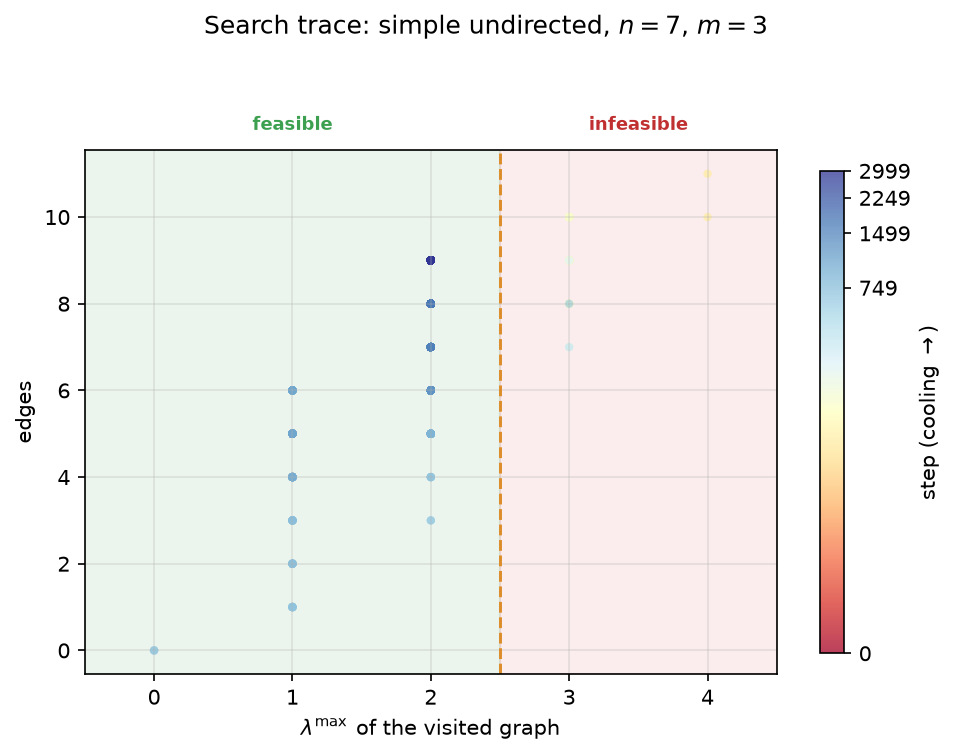
\includegraphics[width=0.74\textwidth]{figures/trace_simple_undirected_n7_m3.png}
    \caption{Search trace for the simple undirected edge problem at $n = 7$, $m = 3$. File \code{trace\_simple\_undirected\_n7\_m3.png}.}
    \label{fig:trace-simple-undirected}
\end{figure}

\begin{figure}[htbp]
    \centering
    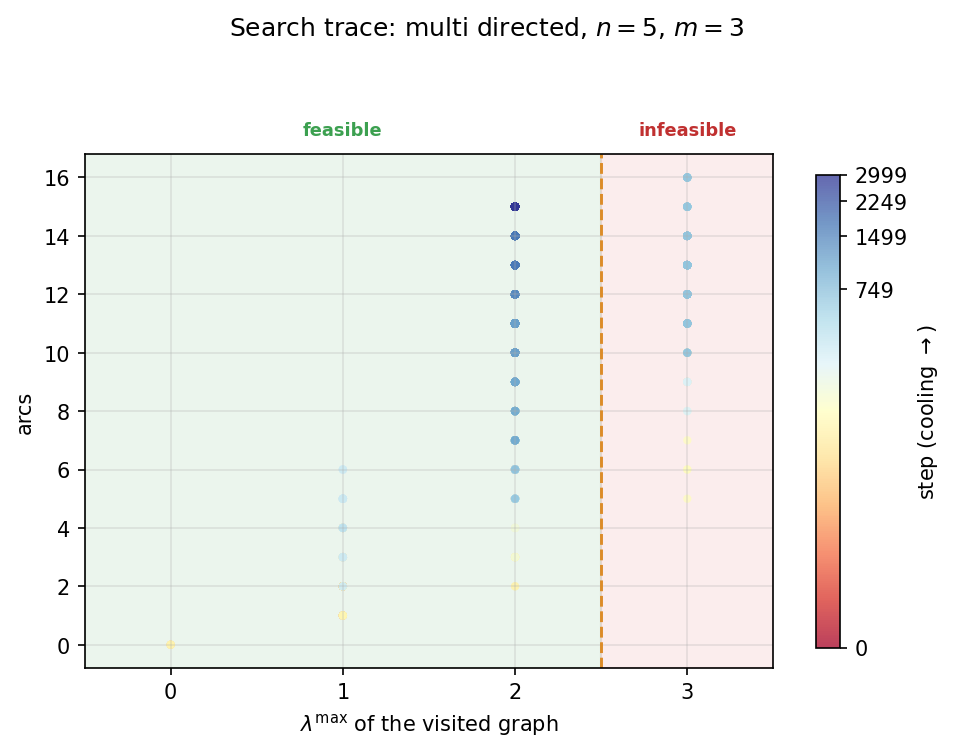
\includegraphics[width=0.74\textwidth]{figures/trace_multi_directed_n5_m3.png}
    \caption{Search trace for the multigraph directed arc problem at $n = 5$, $m = 3$. File \code{trace\_multi\_directed\_n5\_m3.png}.}
    \label{fig:trace-multi-directed}
\end{figure}

\begin{figure}[htbp]
    \centering
    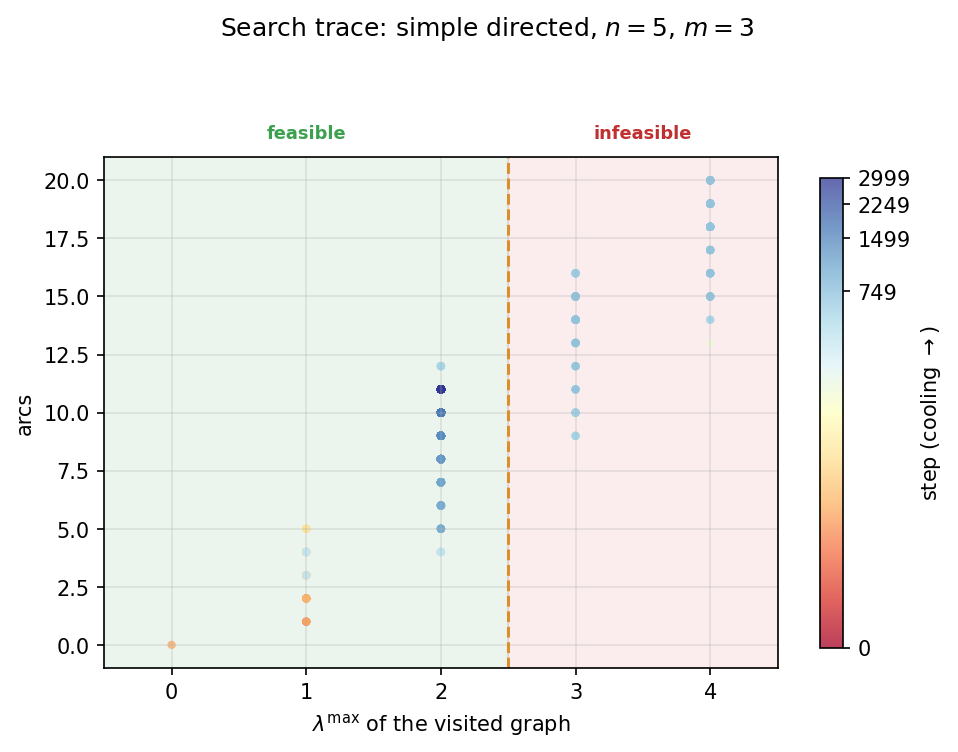
\includegraphics[width=0.74\textwidth]{figures/trace_simple_directed_n5_m3.png}
    \caption{Search trace for the simple directed arc problem at $n = 5$, $m = 3$. File \code{trace\_simple\_directed\_n5\_m3.png}.}
    \label{fig:trace-simple-directed}
\end{figure}

\begin{figure}[htbp]
    \centering
    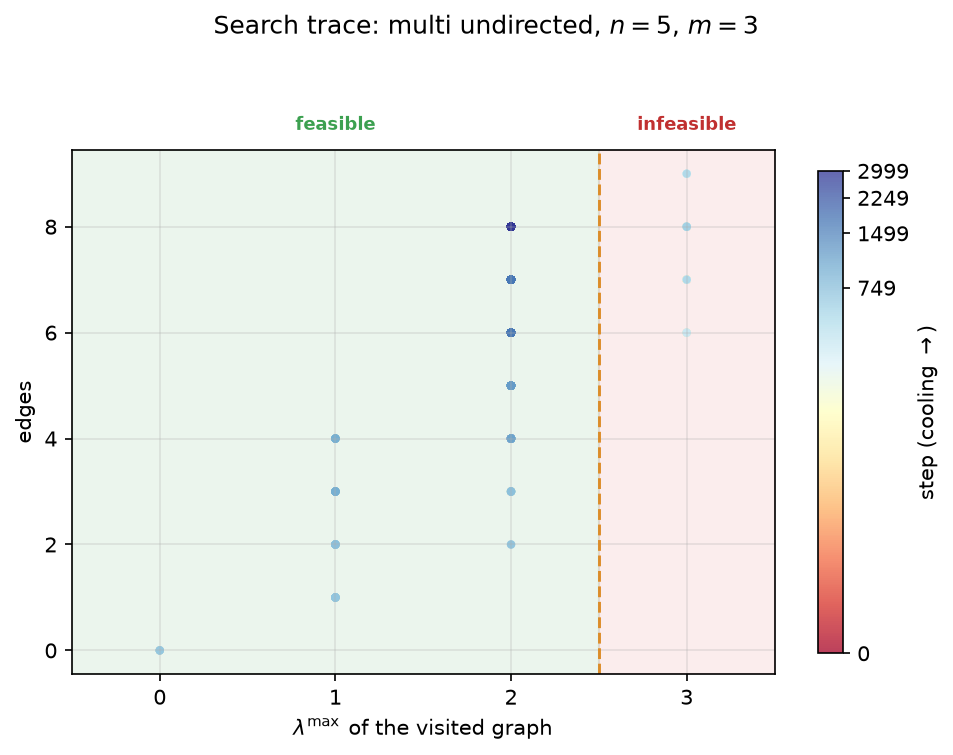
\includegraphics[width=0.74\textwidth]{figures/trace_multi_undirected_n5_m3.png}
    \caption{Search trace for the multigraph undirected edge problem at $n = 5$, $m = 3$. File \code{trace\_multi\_undirected\_n5\_m3.png}.}
    \label{fig:trace-multi-undirected}
\end{figure}

\begin{figure}[htbp]
    \centering
    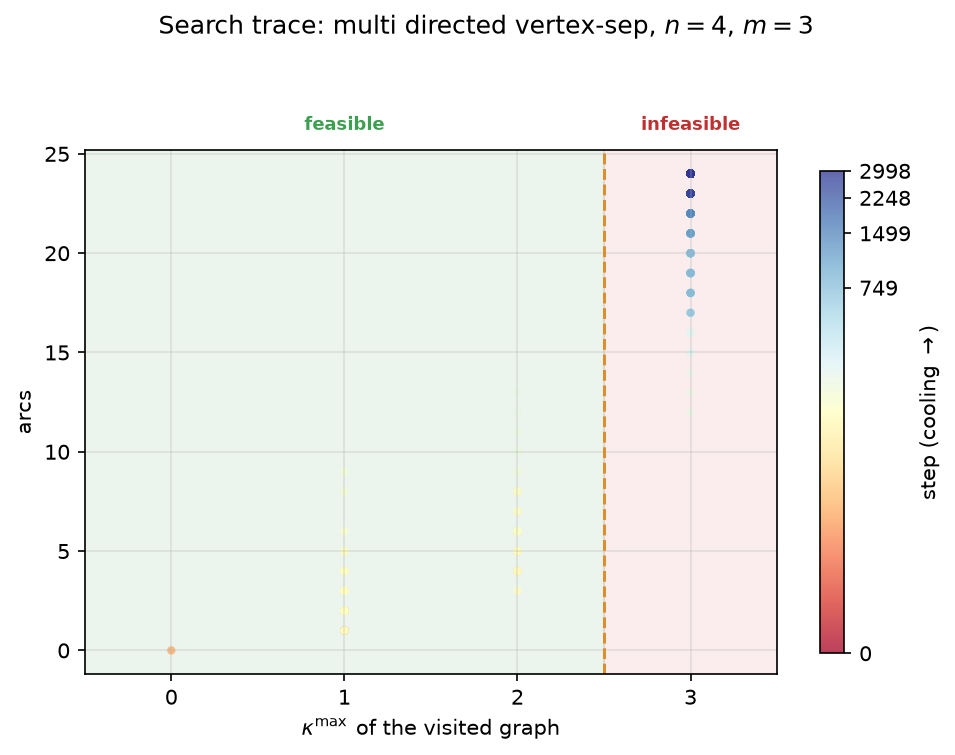
\includegraphics[width=0.74\textwidth]{figures/trace_multi_directed_n4_m3_vertex.png}
    \caption{Search trace for the multigraph directed problem at $n = 4$, $m = 3$ under the \emph{vertex} separation, so the horizontal axis is $\kap^{\max}$ rather than $\lec^{\max}$. This trace spends more of its sampled steps above its own feasibility boundary than the $n = 5$ arc traces above do above theirs, though the mismatched $n$ means the two are not a controlled comparison, and Whitney's inequality in fact makes the vertex-feasible family the larger of the two (\Cref{rem:whitney-direction}). File \code{trace\_multi\_directed\_n4\_m3\_vertex.png}.}
    \label{fig:trace-multi-directed-vertex}
\end{figure}
\end{offcut}

\begin{offcutrewrite}{A1 (repair). The pointer to Appendix B.2 in Chapter 3}{A1}{chapters/ch3\_discover.tex, closing sentence of the temperature-and-sensitivity section}{the walk crystallises onto an extremal shape, before the paragraph ends}{The sentence pointed at a section that no longer exists. Rewritten to keep the fact, drop the pointer.}
This is exactly the behaviour one wants, and it is the behaviour the formulation asks for: the temperature tracks how strongly removing an edge changes the bound. \Cref{fig:trace} shows one such run settling onto a certified optimum. \Cref{app:traces} collects five further traces, covering both matrix models in both directions and one run under the vertex separation, and the behaviour is the same in each.
\nowreads
This is exactly the behaviour one wants, and it is the behaviour the formulation asks for: the temperature tracks how strongly removing an edge changes the bound. \Cref{fig:trace} shows one such run settling onto a certified optimum, and runs across the other matrix models, both directions and the vertex separation behave the same way.
\end{offcutrewrite}

\begin{offcut}{A2 and C3. Appendix B.3, the $m = 6$ distribution and the three-dimensional threshold}{A2, C3}{chapters/app\_gallery.tex, whole section: \code{conn\_dist\_m6.png} and \code{threshold\_3d.png}}{\textbackslash{}label\{fig:extremal-gallery\}, after Group A1 has been restored}{The $m=6$ distribution was referenced only from the gallery itself. The three-dimensional threshold is a fixed $m=3$ experiment, outside the asymptotic regime of \Cref{thm:gnp-threshold}, so placing it beside that theorem would imply support it cannot give.}
\section{The variant landscape at \texorpdfstring{$m = 6$}{m = 6} and in three dimensions}\label{app:m6}

This appendix shows the per-graph connectivity distribution at the fixed forbidden threshold $m = 6$, alongside a three-dimensional view of the appearance threshold (\Cref{fig:threshold-3d}). They confirm that raising the forbidden threshold relocates the feasibility boundary without changing the qualitative picture. The pooled pair-connectivity and edge-count grids of \Cref{ch:synthesis} (\Cref{fig:pair-conn-dist,fig:edge-dist}) already split each variant at its own mid-range connectivity, so they carry no separate $m = 6$ companion.

\begin{figure}[htbp]
    \centering
    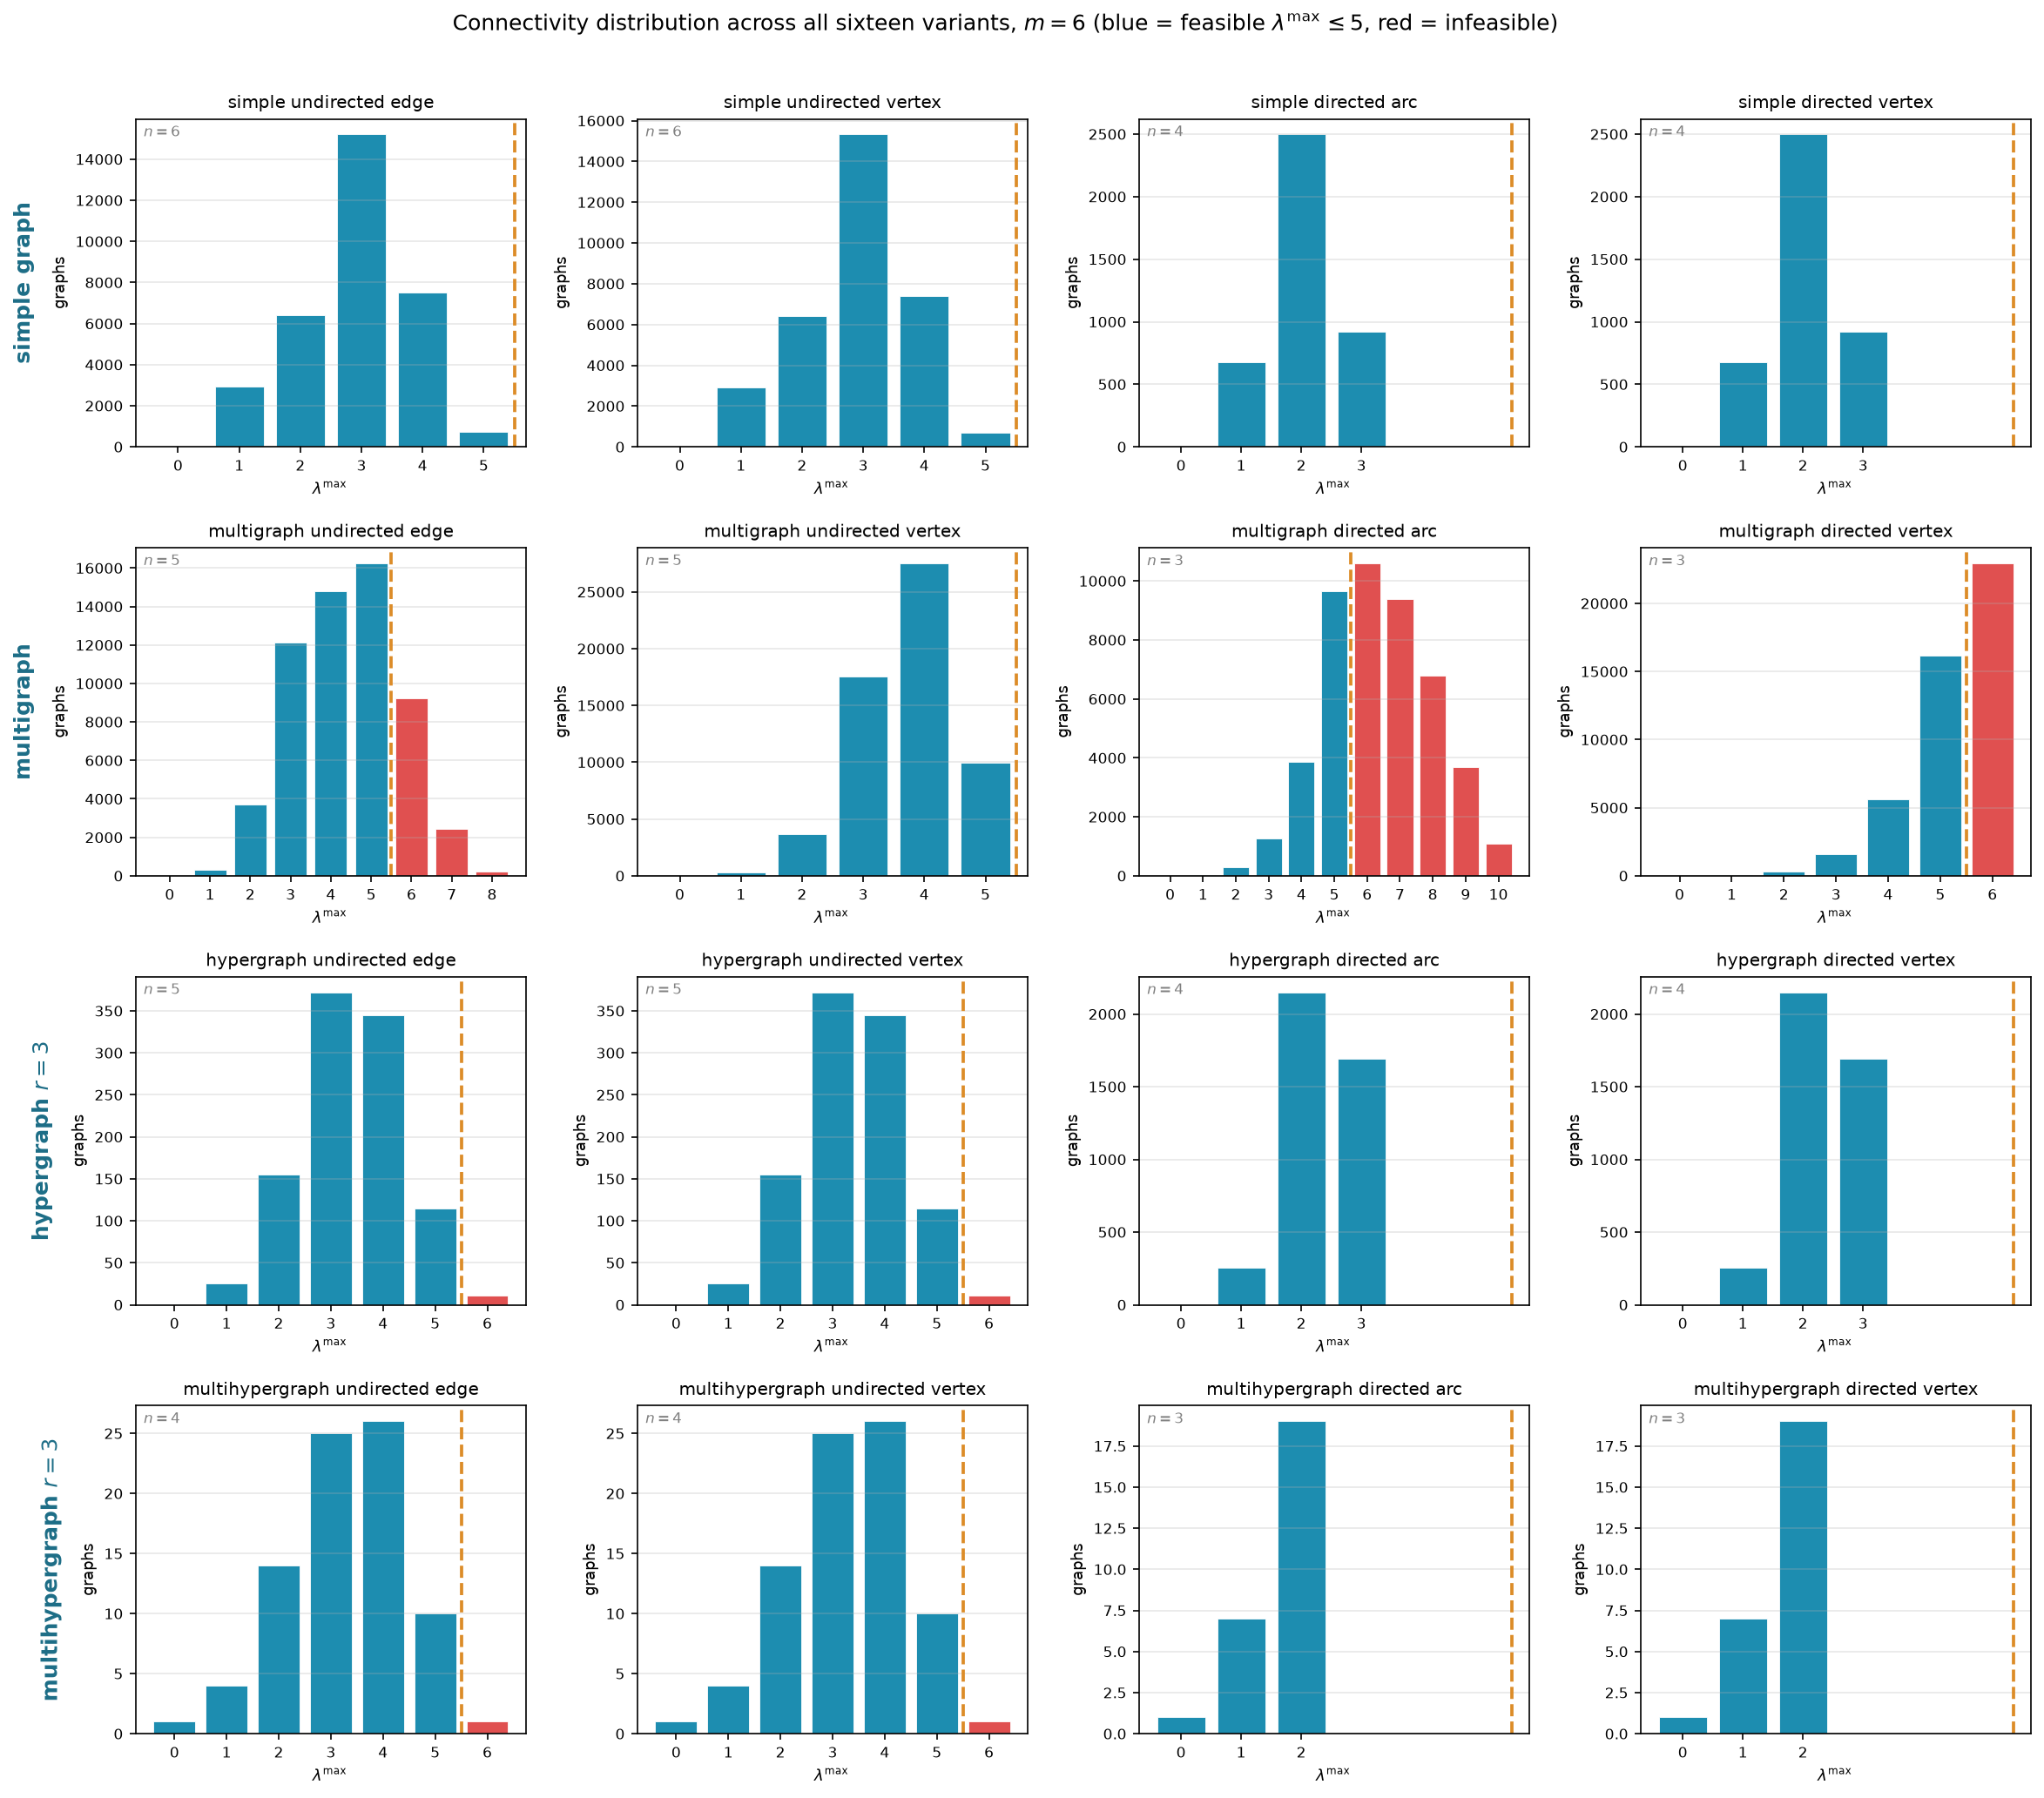
\includegraphics[width=\textwidth]{figures/conn_dist_m6.png}
    \caption{How the full small-$n$ enumeration distributes by binding connectivity $\lambda^{\max}$ across all twelve variants at the fixed forbidden threshold $m = 6$. Blue bars are feasible graphs ($\lambda^{\max} \le 5$), red bars infeasible ones, and the dashed line marks the feasibility boundary. At this higher threshold most of the small graphs the enumeration reaches are feasible, so the blue mass dominates: raising $m$ moves the boundary out past the bulk of the distribution. File \code{conn\_dist\_m6.png}.}
    \label{fig:conn-dist-m6}
\end{figure}

\begin{figure}[htbp]
    \centering
    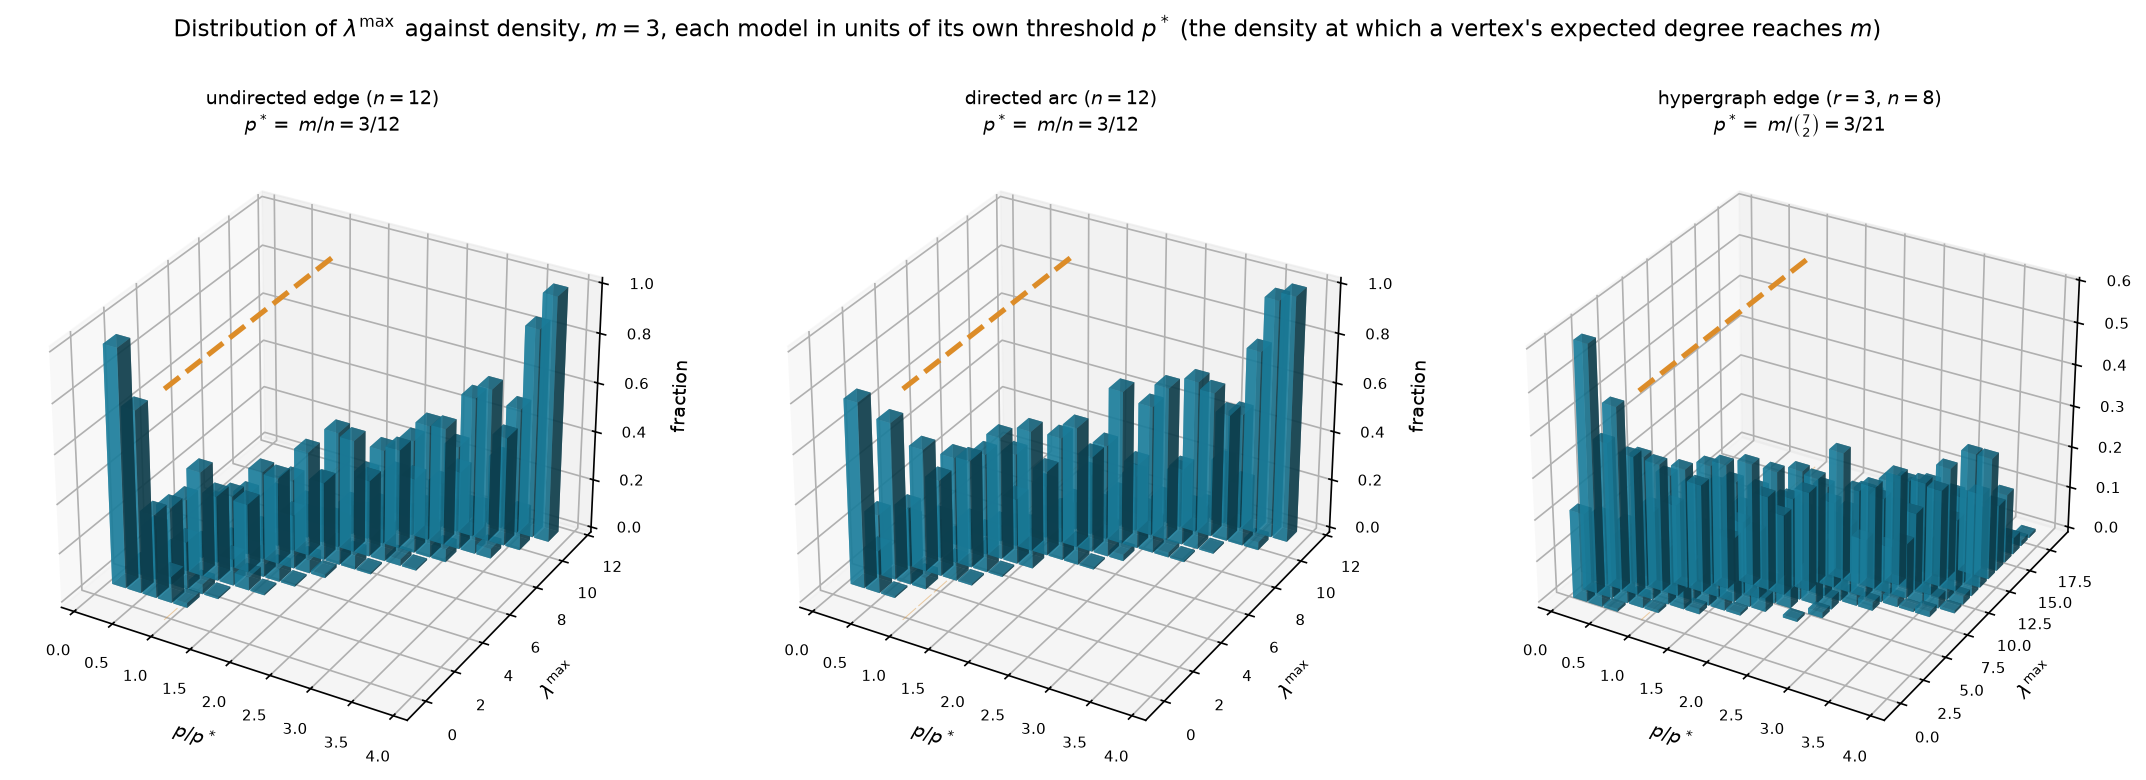
\includegraphics[width=0.86\textwidth]{figures/threshold_3d.png}
    \caption{A three-dimensional sampling experiment for three representative variants (simple undirected edge and simple directed arc at $n = 12$, three-uniform hypergraph edge at $n = 8$), all at $m = 3$. Each panel plots the fraction of samples (height) reaching each binding connectivity $\lambda^{\max}$ (depth) against density (width), and the mass migrates from low to high connectivity near the dashed degree-balance scale. The models do \emph{not} share a density scale: the guide is $m/n$ for the two graph models and $m/\binom{n-1}{r-1}$ for the hypergraph. Only the undirected graph panel corresponds to the model of \Cref{thm:gnp-threshold}, and the directed and hypergraph panels are empirical comparisons, not consequences of that theorem. Moreover, all three panels use fixed $m=3$ and therefore lie outside its asymptotic regime $m/\ln n\to\infty$. The figure illustrates behaviour at small parameters and does not establish a threshold for either unsupported model. File \code{threshold\_3d.png}.}
    \label{fig:threshold-3d}
\end{figure}
\end{offcut}

\begin{offcut}{A3. The two population distributions}{A3}{chapters/ch4\_synthesis.tex, \code{pair\_conn\_dist.png} and \code{edges\_dist.png}, two full-page floats}{the extremal envelope paragraph ending ``a thin frontier with almost nothing pressed against it from below.''}{Both make the same point, that dense low-connectivity graphs are rare, and that point would hold for any extremal problem. \Cref{fig:scatter-landscape} and \Cref{fig:surface-3d} stay: the first carries the extremal envelope, the second separates proved values from search lower bounds.}
\begin{figure}[p]
    \centering
    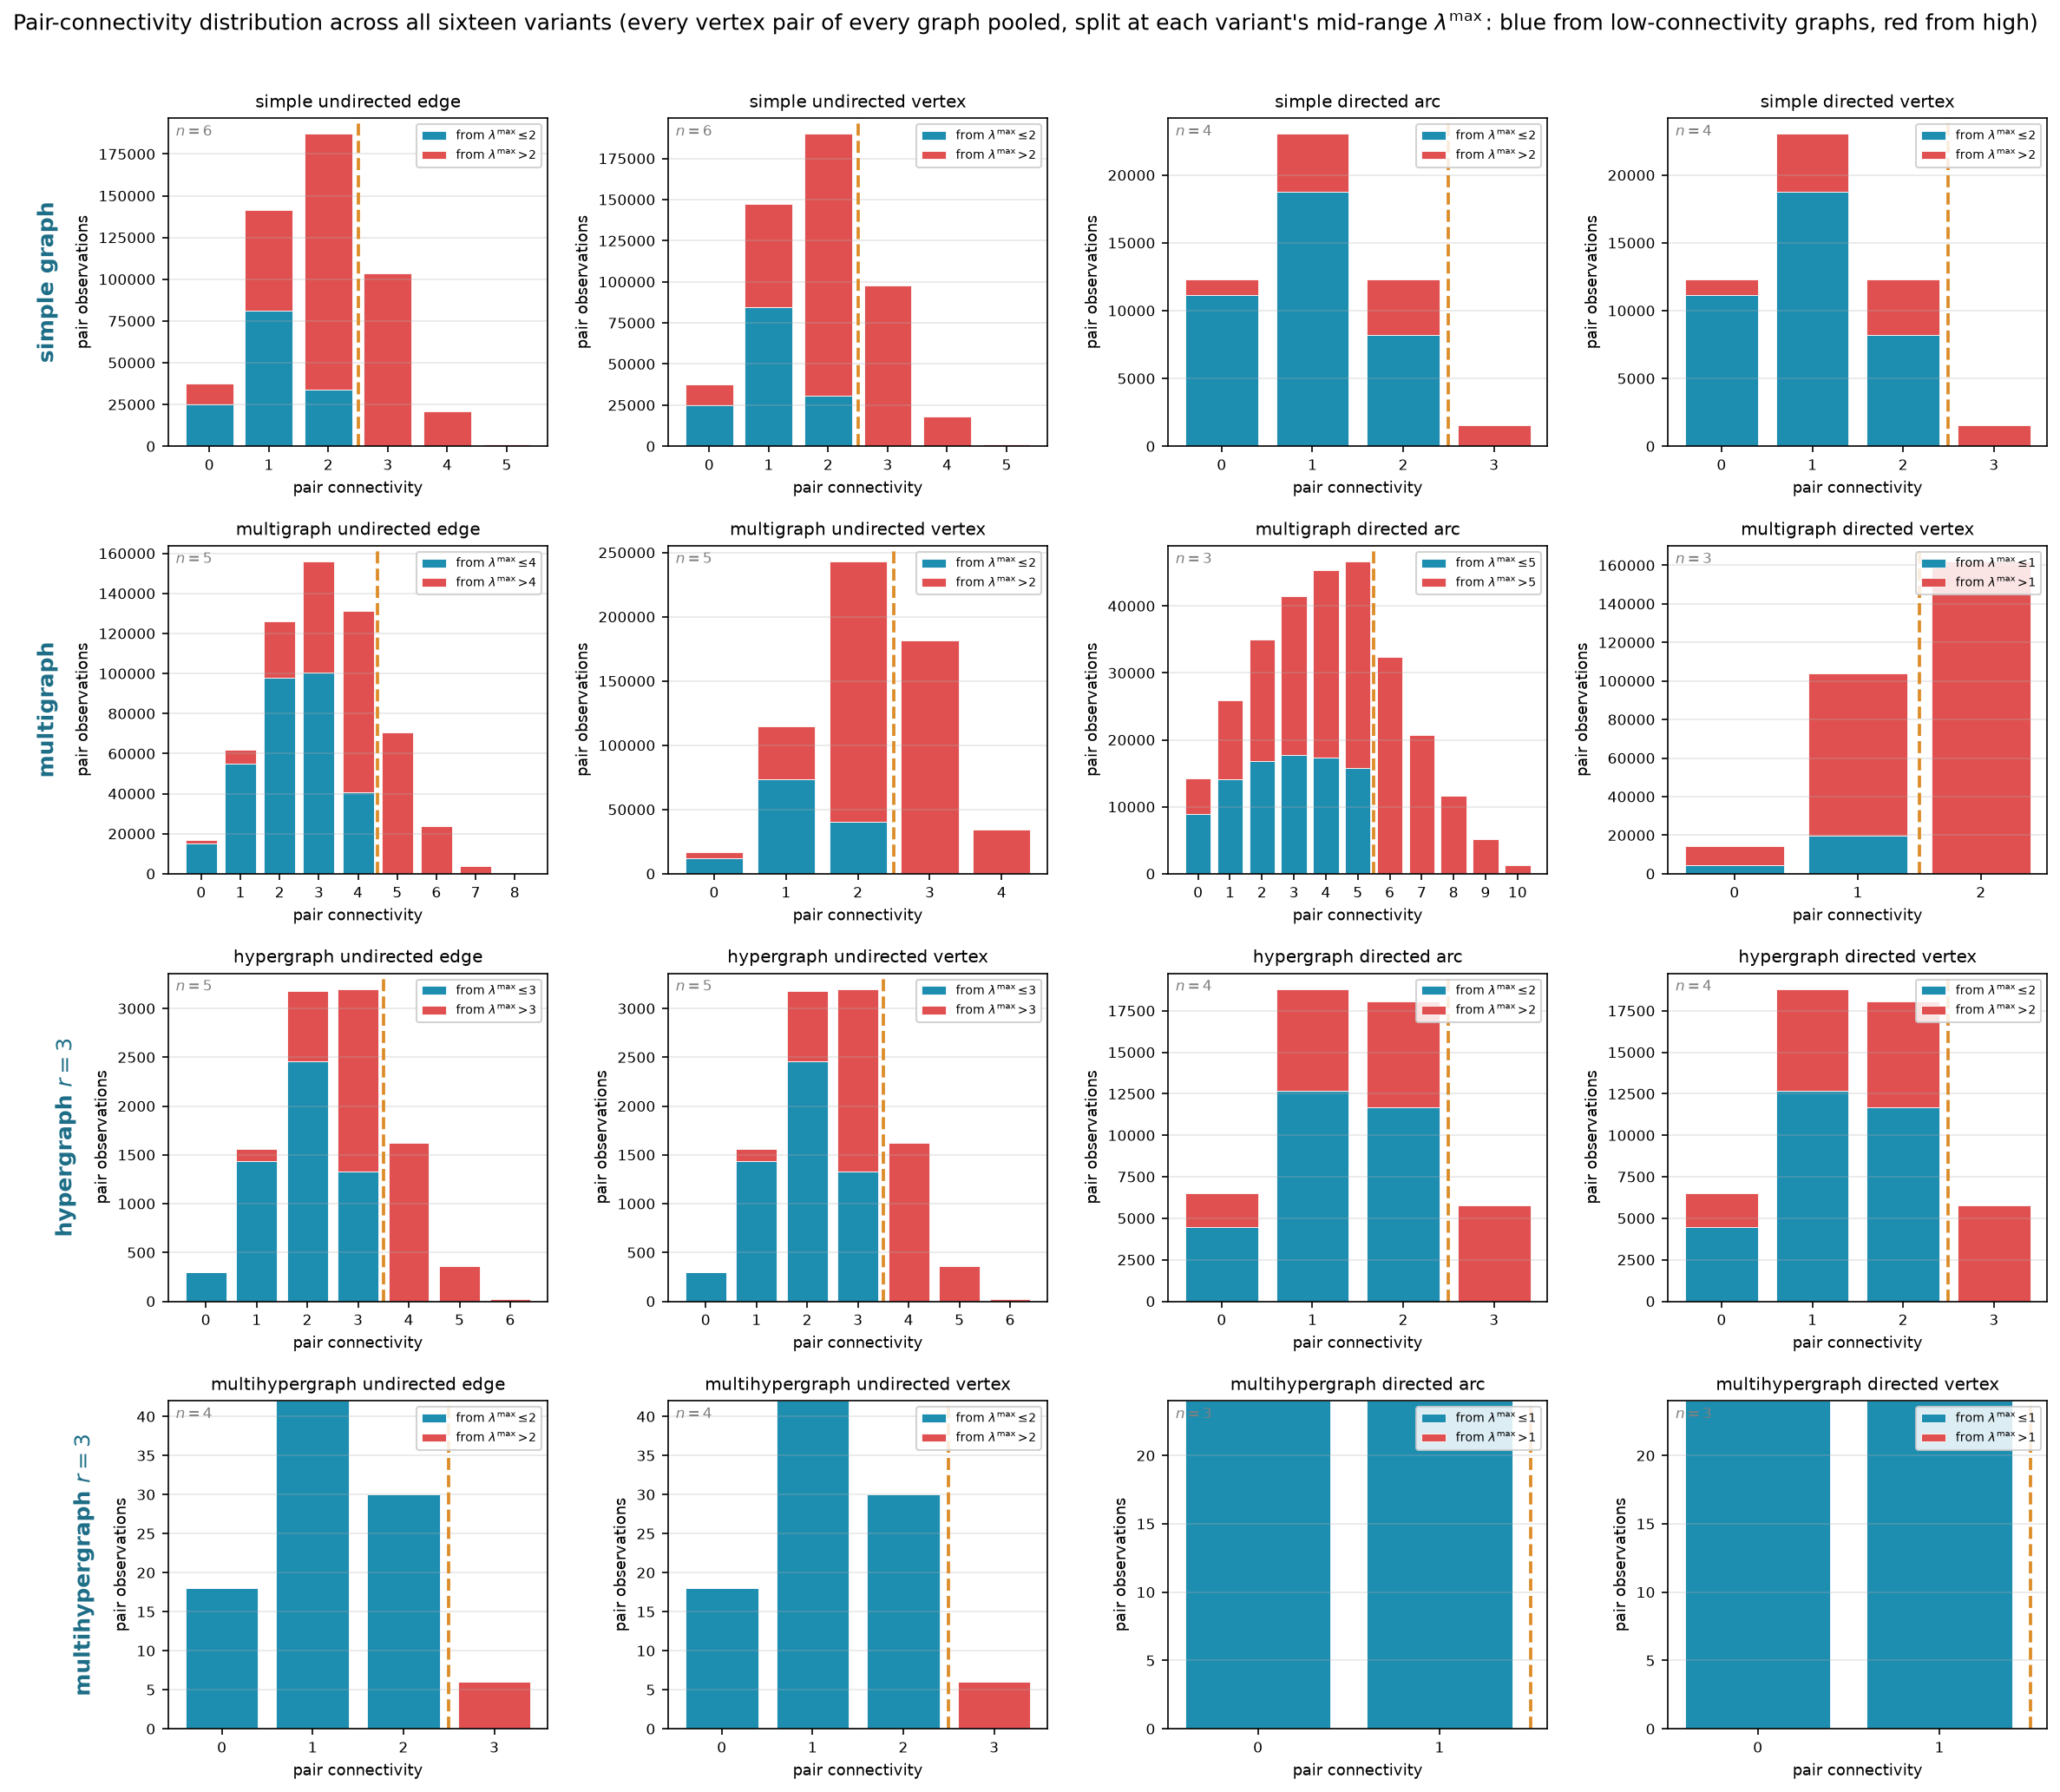
\includegraphics[width=\textwidth]{figures/pair_conn_dist.png}
    \caption{Pair-connectivity distribution across all twelve variants, pooling every vertex pair of every graph in the full enumeration. The horizontal axis is the connectivity of a single pair, and a bar's height is the number of (graph, pair) observations at that level. Each bar is split and stacked by the connectivity of the graph the pair was drawn from, blue from graphs at or below a per-panel boundary $T$ and red from graphs above it, with the dashed line at $T$. The boundary is set per variant to the midpoint of the connectivity range that variant's enumeration reaches (each panel's legend gives its $T$), so the split stays informative in every panel instead of collapsing to one colour. Bars to the right of the dashed line are wholly red, since a pair of connectivity above $T$ forces its graph above $T$. To the left the colours mix.}
    \label{fig:pair-conn-dist}
\end{figure}

\begin{figure}[p]
    \centering
    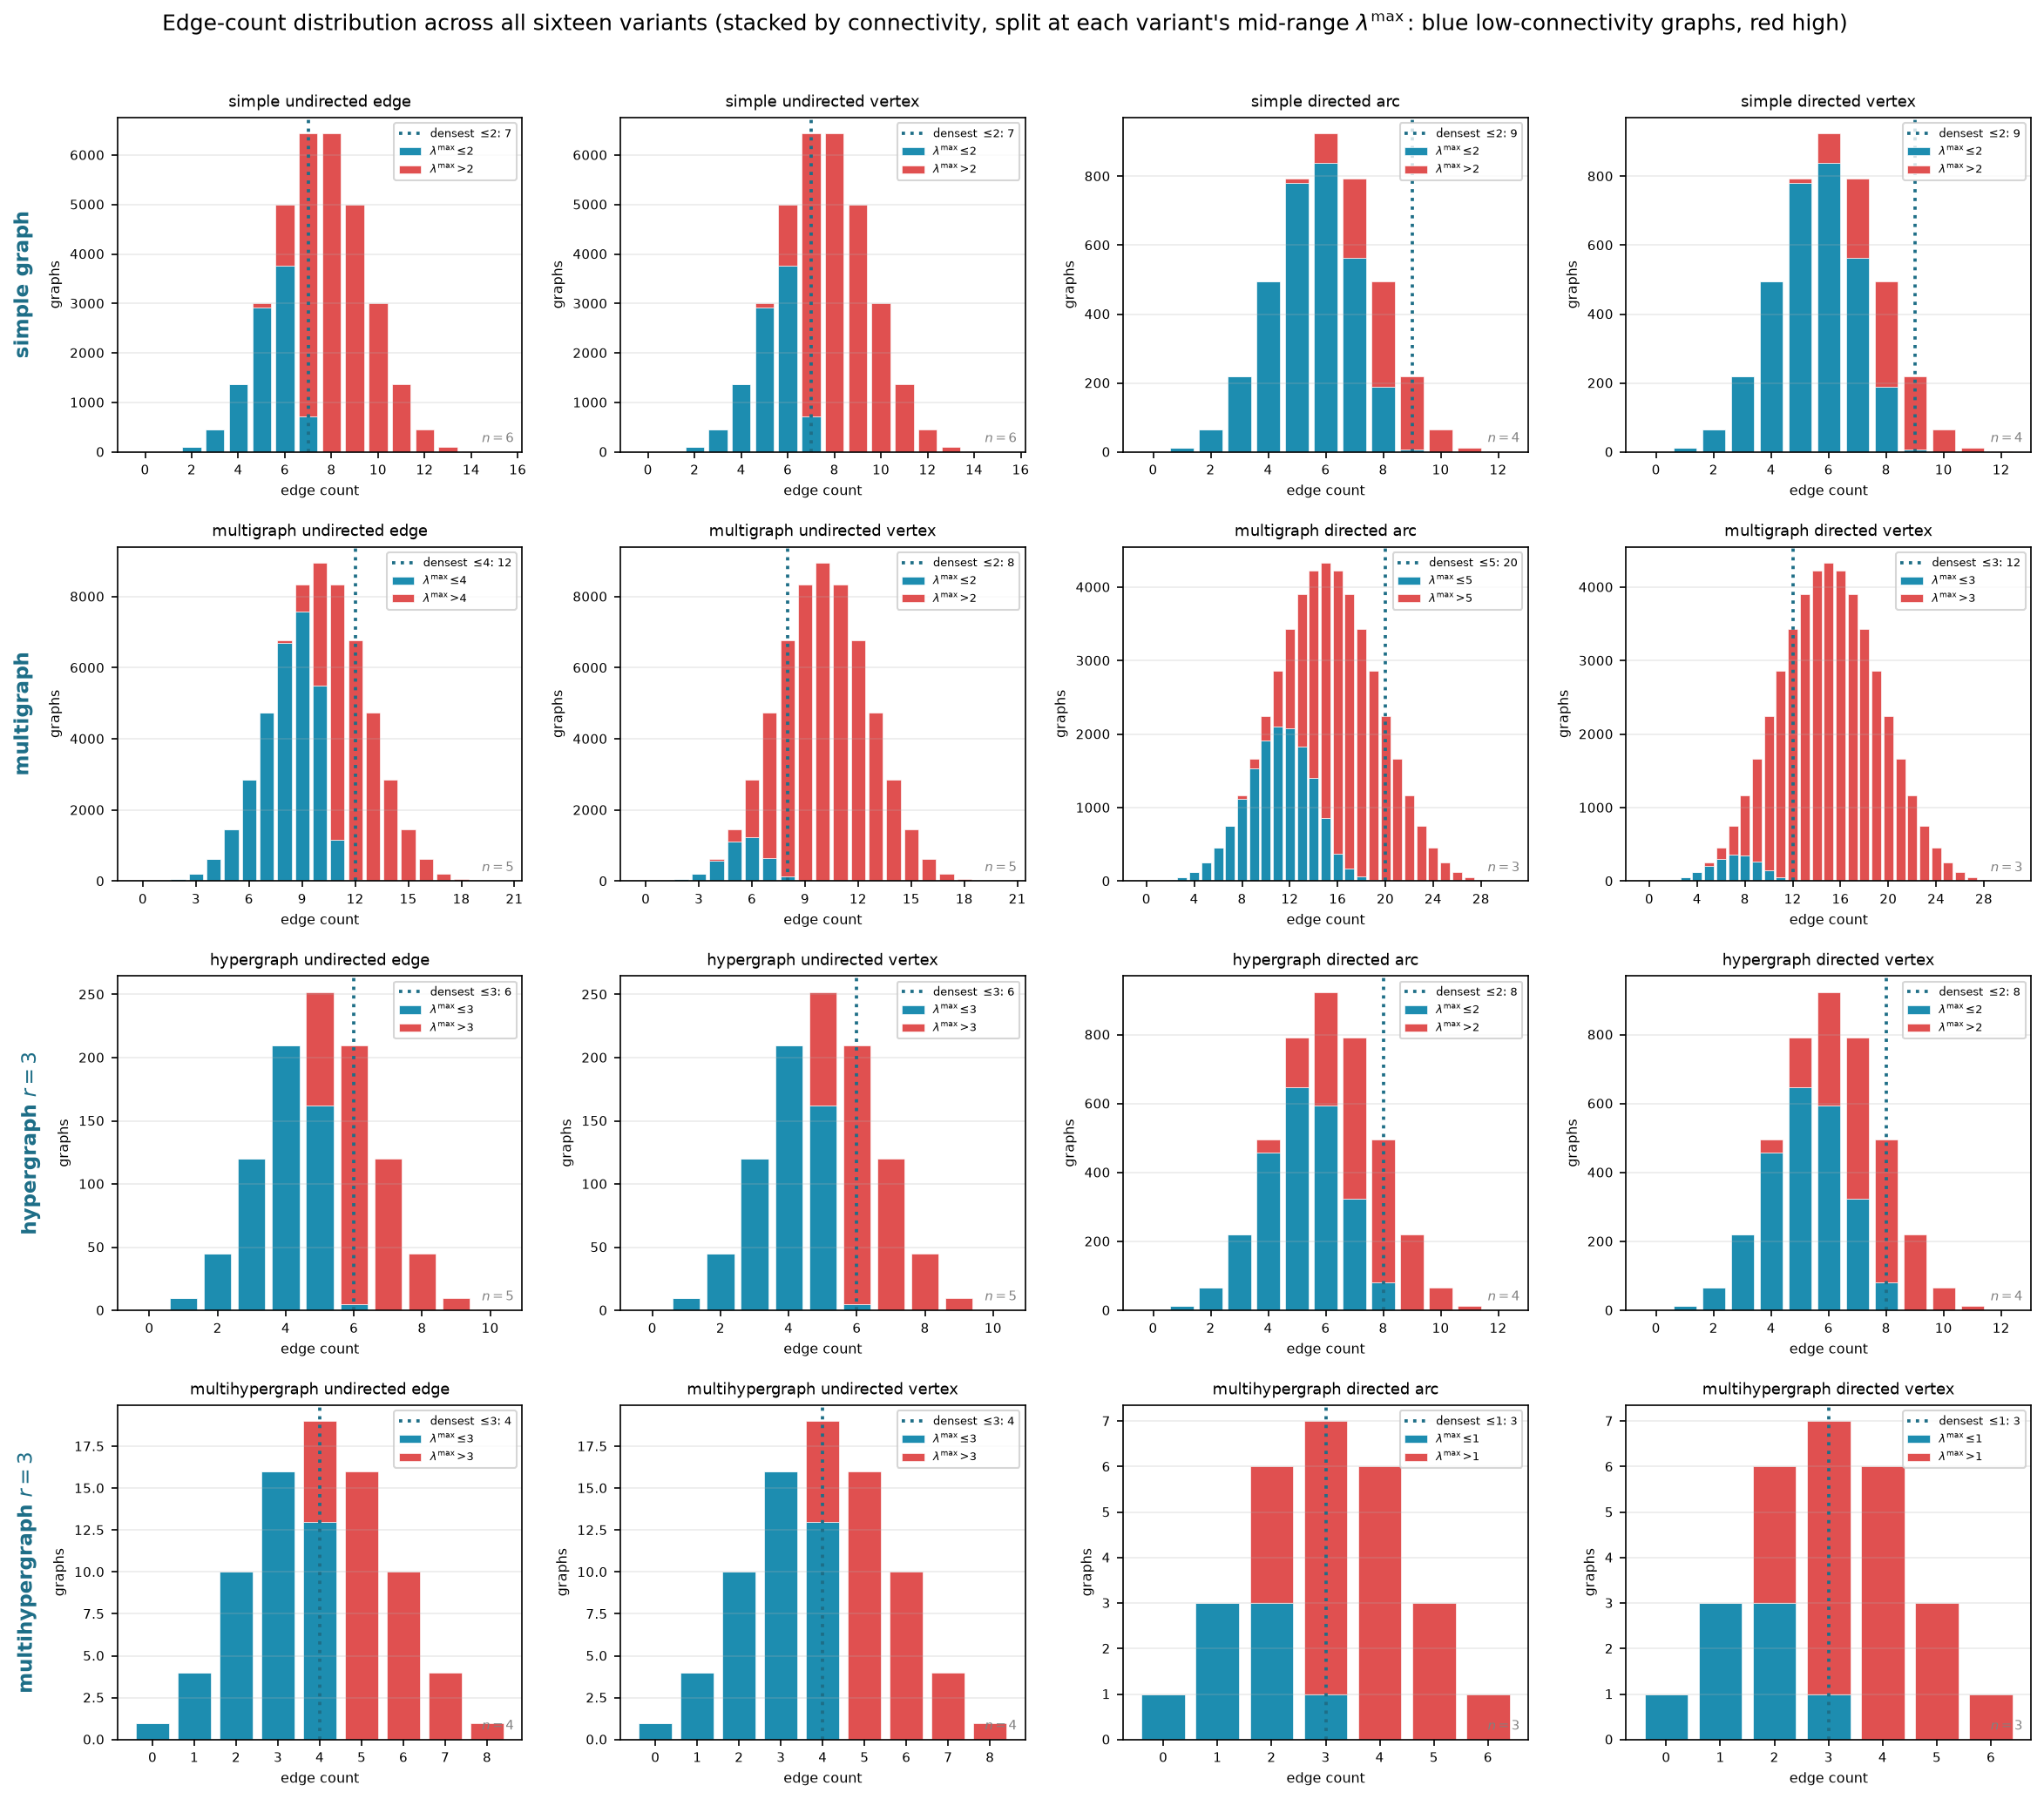
\includegraphics[width=\textwidth]{figures/edges_dist.png}
    \caption{Edge-count distribution across all twelve variants, the same enumeration viewed by edge count rather than connectivity. Each bar is split and stacked by graph connectivity, blue for graphs at or below the per-panel boundary $T$ and red above it (each panel's legend gives its $T$), so the full height is the total number of graphs at that edge count. The dotted vertical line marks the densest graph on the low-connectivity side. The reader can see directly how the two populations separate by edge count and how far the densest low-connectivity graphs sit from the bulk.}
    \label{fig:edge-dist}
\end{figure}
\end{offcut}

\begin{offcutrewrite}{A3 (prose). The two paragraphs describing those figures}{A3}{chapters/ch4\_synthesis.tex, two paragraphs in the phenomena section}{the same anchor as A3 above}{Orphaned once the figures moved. Compressed to one sentence that keeps both observations.}
\Cref{fig:pair-conn-dist} steps inside each graph to the level of individual pairs. For every graph in the full enumeration it records the connectivity of every vertex pair and pools all the observations, so the histogram counts not graphs but (graph, pair) observations. Each bar is split and stacked by the connectivity of the graph the pair came from: blue for pairs drawn from the lower-connectivity graphs, red for pairs from the higher-connectivity ones. The boundary between the two is set per variant at the midpoint of the connectivity range that variant's enumeration can reach, since the twelve variants span very different ranges and a single fixed boundary would leave some panels entirely one colour. A pair whose own connectivity exceeds the boundary can only come from a graph above it, so the bars to the right of the dashed line are wholly red, while to the left the two colours mix, since a high-connectivity graph still carries many low-connectivity pairs. The blue mass sits almost entirely at the lowest levels: high-connectivity pairs are rare even inside the graphs that have one.

\Cref{fig:edge-dist} then shows how the same graphs distribute by sheer edge count, with the same per-variant stacked colouring. At each edge count the blue part counts the lower-connectivity graphs and the red part the higher-connectivity ones, so the bar height is the total number of graphs there and the split shows how the two populations separate. The red mass sits to the right, since denser graphs tend to carry higher connectivity, and the dotted line marks the densest graph still on the low-connectivity side, landing far out in the sparse tail. The densest low-connectivity graphs, the ones the extremal problem is about, are exceptional in every variant.
\nowreads
Pooling the same enumeration by individual vertex pair and by sheer edge count tells the same story from two more angles: high-connectivity pairs are rare even inside the graphs that have one, and the densest low-connectivity graphs, the ones the extremal problem is about, sit far out in the sparse tail in every variant.
\end{offcutrewrite}

\begin{offcutrewrite}{A4. Section 2.9, ``Reproducibility''}{A4}{chapters/ch2\_certify.tex, three paragraphs}{the section heading \textbackslash{}section\{Reproducibility\}}{Duplicated \Cref{app:code} line for line. Replaced by a bridge to it.}
Every claim in this thesis that rests on computation can be re-run from a single Python driver. All of the program's logic lives in \code{program/erdos915\_unified.py}, one self-contained file. Its core needs only \code{numpy} and \code{scipy}, because every connectivity value it reports is a single \code{scipy} integer maximum flow on a capacity matrix. The model, the checker, the search, the enumeration, and the self-test all run on those two libraries alone.

A few more libraries sit on top, each for one job. The certifier uses \code{pulp}, a Python library for writing an optimisation once and handing it to any solver, and runs it on CBC, the free solver \code{pulp} bundles, or on the commercial Gurobi solver by a one-line switch. Two others are optional and only for presentation: \code{matplotlib} draws the figures, and \code{networkx} supplies the Gomory--Hu tree behind one of them. An optional compiled helper, \code{\_erdos\_fast.so} (built from \code{\_erdos\_fast.c} by \code{build\_fast.sh}), speeds up the hot-path \code{\_tiny\_maxflow} and \code{\_canonical\_form} calls, but the pure-Python path returns the same answers.

A handful of named entry points reach the whole pipeline. \code{solve} drives every variant. The measures are \code{max\_edge\_connectivity} and \code{max\_vertex\_connectivity}, with the hypergraph and Gomory--Hu views beside them. The provers are \code{prove\_directed\_multigraph} and \code{enumerate\_extremal\_directed\_multigraphs}, and \code{search\_for\_dense\_graph} is the discoverer. Running \code{python erdos915\_unified.py} executes the built-in self-test, the suite of invariant checks that confirms the connectivity values quoted throughout this chapter, including the sanity checks on the bidirected star and on $K_n$ and $K_4^{(3)}$.

The figures and finite outputs are reproducible as well. Every figure is regenerated by the companion driver \code{program/make\_figures.py}, which imports the same file and fixes every random seed, and the table in \code{program/README.md} records which routine produces which figure. The exception is \Cref{fig:sa-vs-tabu}: it is deliberately wall-clock timed and therefore representative rather than seed-exact. Compatible environments reproduce the other numerical data, though image bytes may still differ with plotting libraries, fonts, or compression. The solver transcripts behind this chapter's finite values, the pruned-search log for \Cref{thm:dir-arc-m2-exact} and the cut-counting solver record for \Cref{thm:dir-multi-small}, are reproduced verbatim in \Cref{app:proofs}. The archive, commands, dependency record, and audit protocol are specified in \Cref{app:code}.
\nowreads
Every claim in this thesis that rests on computation re-runs from a single Python driver. All of the program's logic lives in \code{program/erdos915\_unified.py}, one self-contained file whose core needs only \code{numpy} and \code{scipy}, because every connectivity value it reports is one \code{scipy} integer maximum flow on a capacity matrix. \code{pulp} sits on top for the certifier, and \code{matplotlib} and \code{networkx} only for presentation. \Cref{app:code} carries the rest in full: the archive layout, the environment, the named entry points, the commands, the table recording which routine draws which figure, and the archival protocol. The solver transcripts behind this chapter's finite values are reproduced in \Cref{sec:transcripts}.
\end{offcutrewrite}

\begin{offcutrewrite}{A4 (continued). Section 2.9.1, the four practices}{A4}{chapters/ch2\_certify.tex, subsection \code{sec:certification-standard}}{the subsection heading, directly after the bridge above}{The enumeration of what was checked duplicates \Cref{app:verification-ladder} and \Cref{app:software-tests}. The evidential standard itself is kept; the inventory is not.}
Reproducibility is not the same as certification, and it is worth stating plainly what standard the computed results here meet, since a solver reporting \texttt{OPTIMAL} is not by itself a mathematical certificate. Four practices carry the weight.

First, the exhaustive searches are self-certifying in a way the optimisations are not. A finished include-or-exclude sweep has visited a superset of the objects it needed to visit, and the two prunes are proved sound in \Cref{ch:discover}, so its verdict depends on no solver and no floating-point arithmetic, only on the checker. Where a value in this thesis is called \emph{proved}, that is usually the reason.

Second, every reported connectivity is exact and integral. The checker is a single integer maximum flow, so no extremal value in the thesis is a rounded floating-point quantity. Real numbers enter in exactly one place that carries a reported extremal value, the fractional optimisation of \Cref{thm:dir-multi-small}, where the reported optimum is a $\{0,1\}$ matrix and is checked exactly.

Third, the load-bearing computations are run twice, by implementations that share no code. The base cases of \Cref{thm:dir-arc-m2-exact} and \Cref{thm:dir-vertex-m2-exact} were each confirmed by the program and by separately written checkers, agreeing on every size. The values of \Cref{sec:multi-vertex-standard} were computed by the program's routine and by an independent script, agreeing on every cell. The maximum-total-degree-$8$ directed multigraph classification at $n = 7$ (\Cref{rem:n7-classification}) was produced by the generation enumerator and re-verified graph by graph with the exact checker. The integral MILP of this chapter re-proves $L_3^{\mathrm{dir}}(n)$ independently of the fractional route at every $n \le 6$, which is as far as it ever got. At $n = 7$ it timed out, so the value $L_3^{\mathrm{dir}}(7) = 24$ rests on the hand proof of \Cref{app:proofs} alone. The route-counting steps behind \Cref{thm:dir-vertex-linear-error} and \Cref{thm:dir-hyper-constant} were checked the same way before they were written down, over several thousand random digraphs and hypergraphs and every ordered pair in each, by a script that shares no code with this program. Those two are hand proofs and do not need the check to stand, but the check is what caught that both inequalities are attained with equality in real instances, which is how one knows the proof is not throwing anything away. Two implementations agreeing is not a proof, but it is the practical guard against the failure mode a certificate would catch, namely a correct method with a wrong program.

Fourth, the self-test at the foot of the file is a standing regression check on every invariant the text quotes, and it is run after every change to the program.

What this does not amount to is a formally checkable certificate of the kind a SAT solver can emit, such as a resolution proof a small independent verifier could replay. That standard would have been the right one to aim at for $L_3^{\mathrm{dir}}(7) = 24$ had it stayed a solver question, since an INFEASIBLE verdict is exactly the shape of claim a resolution proof records. It did not stay one: \Cref{app:proofs} proves the same statement, and its general case for every $n$ and $m$, by hand, so nothing in this thesis currently rests on an infeasibility verdict that lacks such a proof behind it.
\nowreads
Reproducibility is not the same as certification, and it is worth stating plainly what standard the computed results here meet, since a solver reporting \texttt{OPTIMAL} is not by itself a mathematical certificate. Three practices carry the weight. The exhaustive searches are self-certifying in a way the optimisations are not: a finished include-or-exclude sweep has visited a superset of the objects it needed to visit, and the two prunes are proved sound in \Cref{ch:discover}, so its verdict depends on no solver and no floating-point arithmetic, only on the checker. Where a value in this thesis is called \emph{proved}, that is usually the reason. Every reported connectivity is exact and integral, a single integer maximum flow, so no extremal value in the thesis is a rounded floating-point quantity; real numbers enter in exactly one place that carries a reported extremal value, the fractional optimisation of \Cref{thm:dir-multi-small}, where the reported optimum is a $\{0,1\}$ matrix and is checked exactly. And the load-bearing computations are run twice, by implementations that share no code. Two implementations agreeing is not a proof, but it is the practical guard against the failure mode a certificate would catch, namely a correct method with a wrong program. \Cref{app:verification-ladder} sets out what each kind of computation may legitimately conclude and what evidence it must carry, and \Cref{app:software-tests} records which computations were checked which way.

What this does not amount to is a formally checkable certificate of the kind a SAT solver can emit, such as a resolution proof a small independent verifier could replay. That standard would have been the right one to aim at for $L_3^{\mathrm{dir}}(7) = 24$ had it stayed a solver question, since an INFEASIBLE verdict is exactly the shape of claim a resolution proof records. It did not stay one: \Cref{app:proofs} proves the same statement, and its general case for every $n$ and $m$, by hand, so nothing in this thesis currently rests on an infeasibility verdict that lacks such a proof behind it.
\end{offcutrewrite}

\begin{offcut}{A5. Appendix A.12, ``How the program checks itself''}{A5}{chapters/app\_proofs.tex, whole section, four bullets}{the end of \Cref{sec:transcripts}, at the foot of the appendix}{A self-test coverage list, said in Section 2.9.1 and again in \Cref{app:software-tests}. The fuller verification ladder stays in \Cref{app:code}.}
\section{How the program checks itself}

The invariants are checked by the self-test at the foot of \texttt{erdos915\_unified.py}, run simply with \texttt{python erdos915\_unified.py}. Every check passes, grouped here by what they cover.
\begin{itemize}
    \item \emph{Base values.} The checker against the proven $m = 2$ values $2, 4, 6, 8$, the first three vertex base cases of \Cref{thm:dir-vertex-m2-exact}, and the fast vertex-flow test against the exact checker it stands in for.
    \item \emph{Sampled inequalities.} The counting step and both bounds of \Cref{prop:dir-arc-stability} and \Cref{thm:dir-arc-linear-error} on sampled feasible digraphs, including the high-degree case of the latter's proof, and Whitney's inequality on every sample.
    \item \emph{Constructions.} Two values of the alternative-convention multigraph vertex problem of \Cref{sec:multi-vertex-standard}, including the one that separates it from the edge problem, the named constructions against their predicted sizes and connectivities, and the Gomory--Hu shortcut against brute-force max-flow.
    \item \emph{The checker and driver.} The Berge connectivities of the hypergraph checker, the Monte Carlo appearance threshold, the cut-counting optima for small $n$, the search reaching the certified optimum, and the driver returning the proven value or a feasible witness in each mode.
\end{itemize}
A single companion script, \texttt{make\_figures.py}, regenerates every figure in the thesis from the same file, with the mapping listed in \texttt{program/README.md}.
\end{offcut}

\begin{offcut}{A6. Figure 3.6, the twelve-variant grid at $m = 6$}{A6}{chapters/ch3\_discover.tex, \code{variant\_bounds\_m6.png}}{\textbackslash{}label\{fig:variant-bounds-m3\}, after the $m=3$ grid}{A second full-page grid whose own caption says it shows the same thing scaled. One comparison sentence under the $m=3$ grid carries it.}
\begin{figure}[htbp]
    \centering
    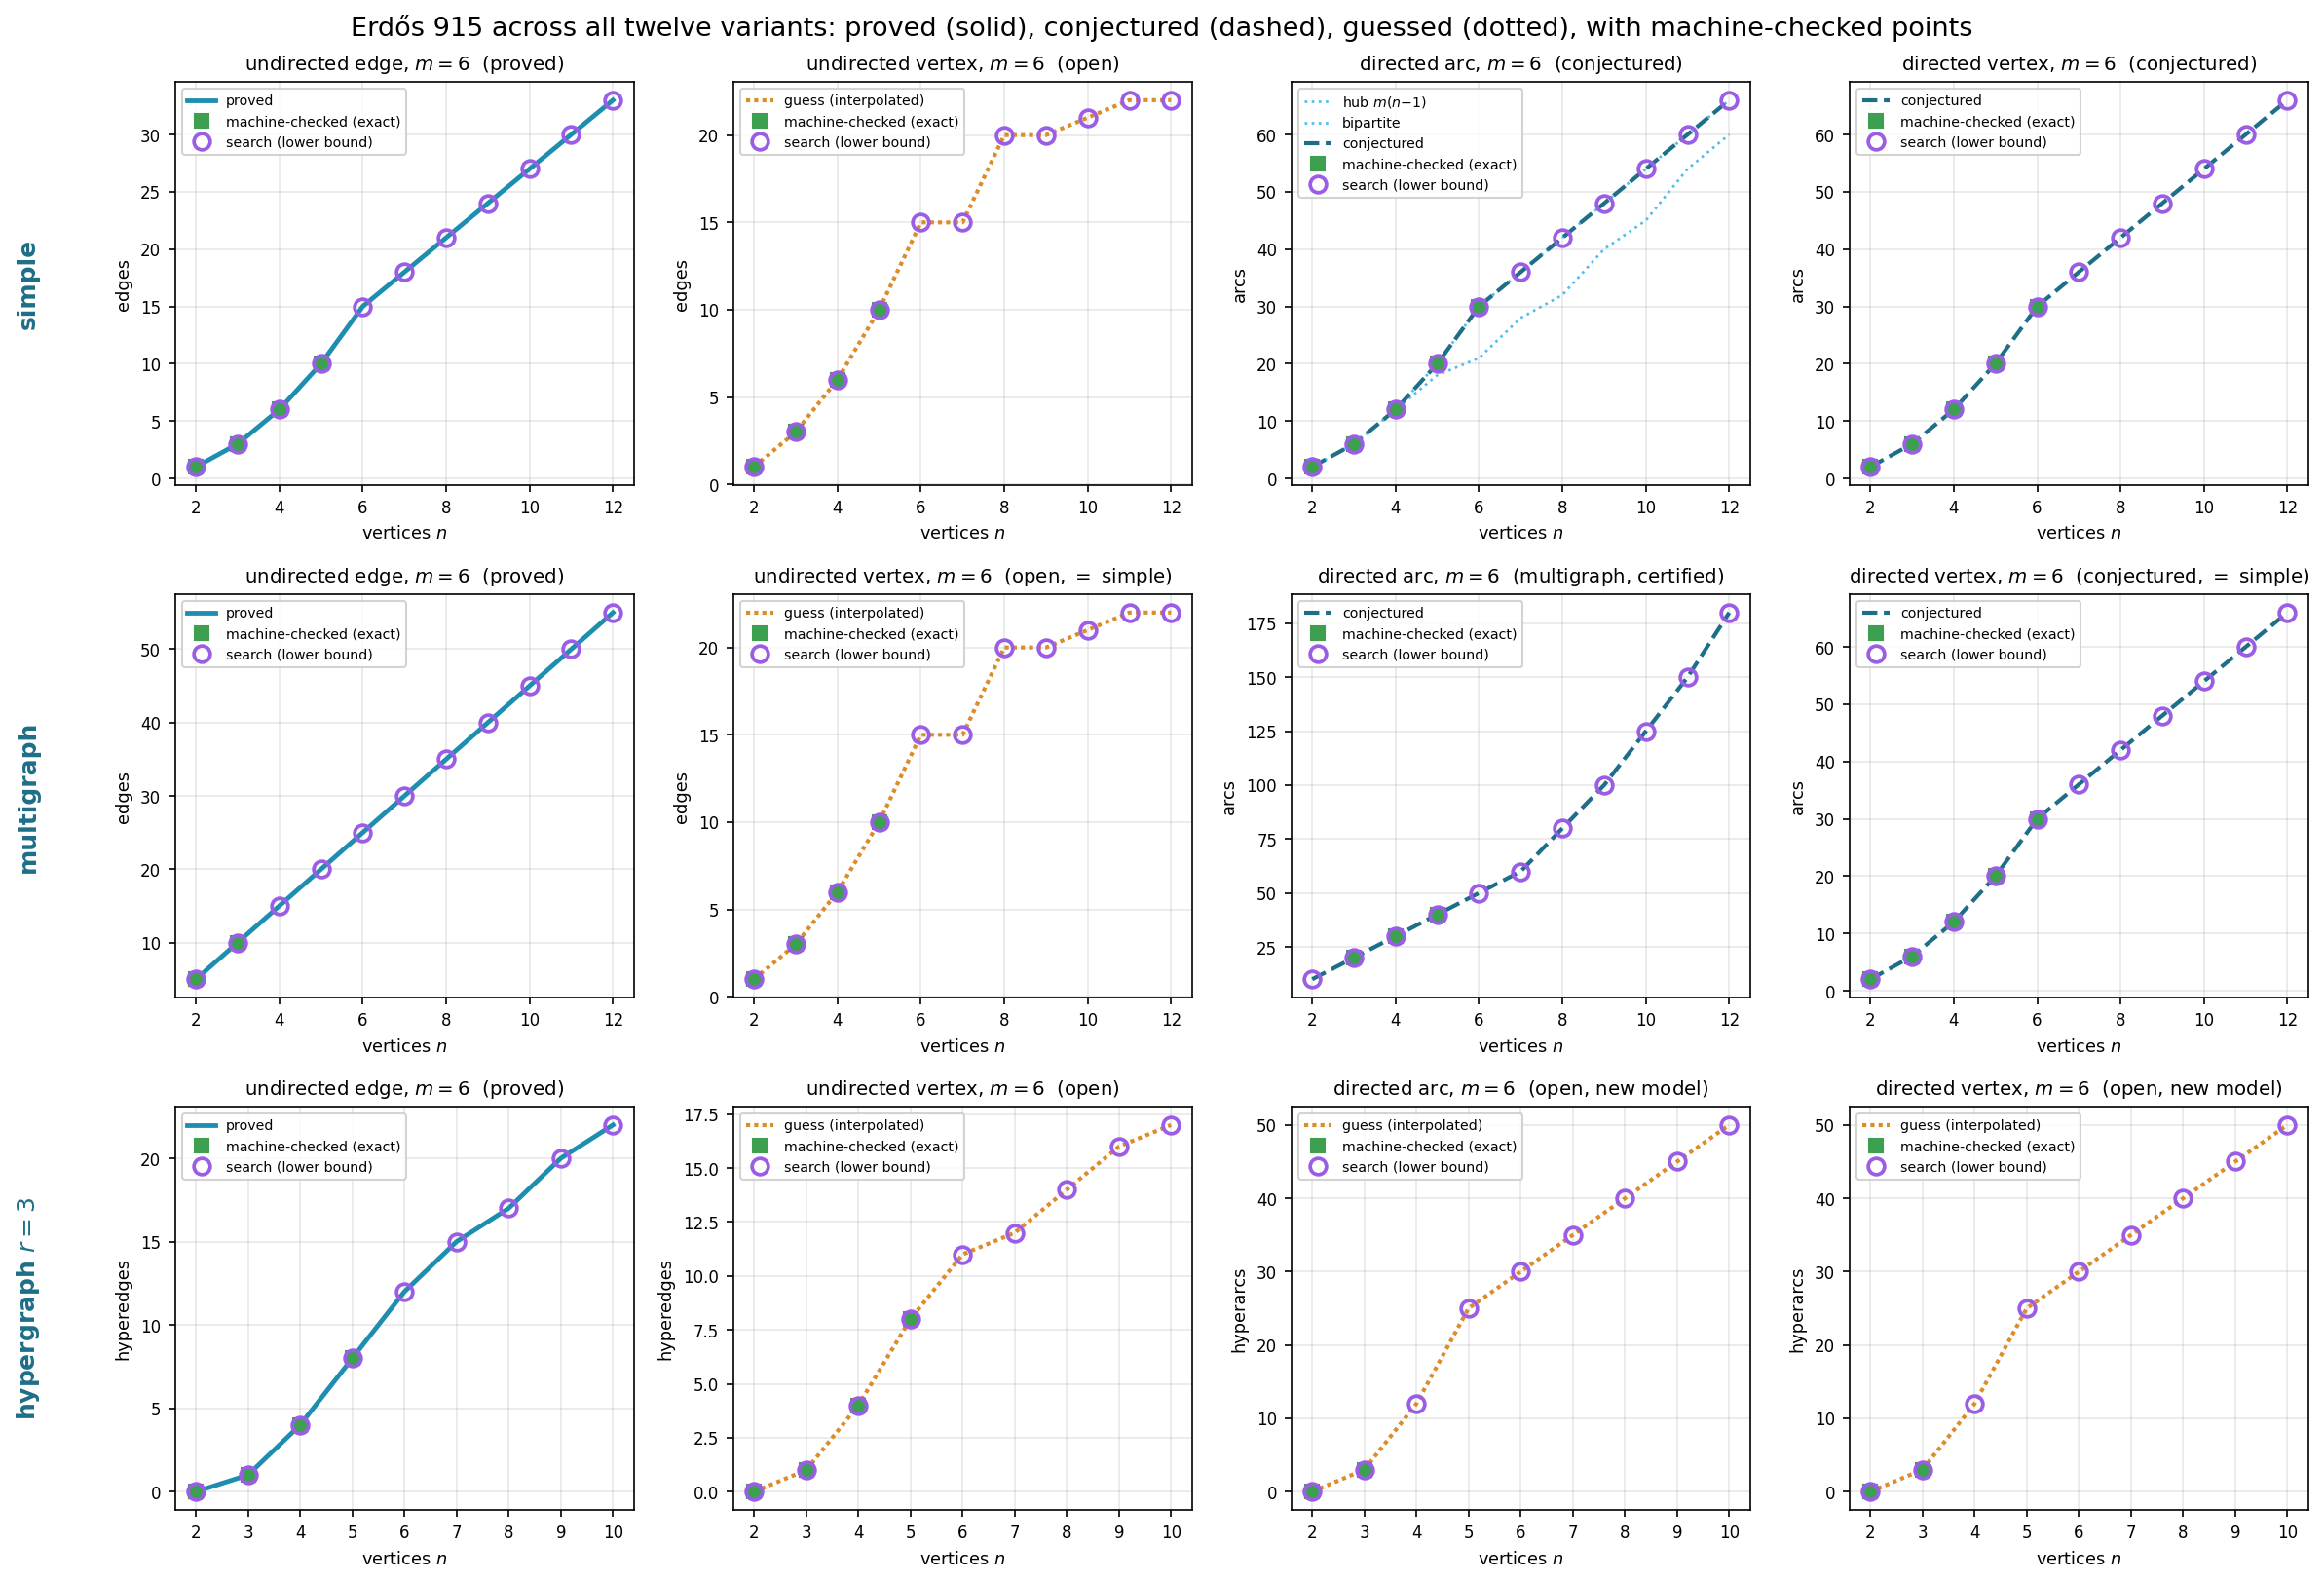
\includegraphics[width=\textwidth]{figures/variant_bounds_m6.png}
    \caption{The same twelve variants at $m = 6$. The undirected edge and multigraph edge cases remain proved (Mader's theorem holds for all $m$), as does the directed multigraph arc case (\Cref{thm:dir-multi-full} holds for all $m$ too), while the undirected vertex separation is the famous open problem at $m \geq 6$ and the directed \emph{simple} cases carry the same conjectured formula scaled to $m = 6$. On the open vertex panels the circles never sit below the proved edge value at the same size. Every graph feasible for the edge problem is feasible for the vertex problem (Whitney), so the edge extremiser is an honest lower bound there, and the search is free to climb past that floor wherever the vertex problem is genuinely richer. Comparing this figure with the $m = 3$ version above shows that the proved cases grow linearly with $m$ as the formulas predict, while on the open cases the circles and their yellow interpolation climb steadily without a proved curve to meet.}
    \label{fig:variant-bounds-m6}
\end{figure}
\end{offcut}

\begin{offcutrewrite}{A6 (prose). The sentences introducing that grid}{A6}{chapters/ch3\_discover.tex, end of the paragraph on directed steepness}{every directed column bends upward while the two undirected columns stay linear.}{Rewritten so the comparison survives without the figure.}
 \Cref{fig:variant-bounds-m6} redraws the same grid at $m = 6$. The proved curves climb linearly with $m$, exactly as their formulas predict, while the open variants' search points and their yellow interpolation climb higher with no proved curve to meet. Raising the threshold therefore does not change which regime a variant lives in, only how far the red and yellow curves have travelled.
\nowreads
 Redrawing the same grid at $m = 6$ changes nothing structural: the proved curves climb linearly with $m$ exactly as their formulas predict, the open variants' search points climb higher with no proved curve to meet, and raising the threshold moves how far the red and yellow curves have travelled rather than which regime a variant lives in.
\end{offcutrewrite}

\section*{Group B: shortened, not deleted}
\addcontentsline{toc}{chapter}{Group B: shortened, not deleted}
\markboth{Group B: shortened, not deleted}{Group B: shortened, not deleted}

\begin{offcutrewrite}{B1. Appendix A.11, the computational transcripts}{B1}{chapters/app\_proofs.tex, three \textbackslash{}lstinputlisting dumps and their lead-ins}{the section heading \textbackslash{}section\{Computational transcripts\}}{The certificate dump goes: it records solver status with no replayable dual certificate or gap, for a value now proved by hand. The two base-case logs are NOT decoration, they are the settled base cases of the directed $m=2$ vertex theorem, so they stay as a compact table.}
The cut-counting optimisation formulation used as a finite solver check for \Cref{thm:dir-multi-small} is given in \Cref{ch:certify}. Here are the historical solver records, together with the exhaustive-search output that settles the directed base cases. The first records solver status but not an independently replayable dual certificate or gap. The theorem itself is proved by hand in this appendix. The complete commented source is maintained with the document as \texttt{erdos915\_unified.py} in the \texttt{program/} directory and should be included in the archived submission described in \Cref{app:code}. Its core runs on \texttt{numpy} and \texttt{scipy} alone, the certifier adds \texttt{pulp}, and \texttt{matplotlib} and \texttt{networkx} are optional analysis and visualisation dependencies. An optional compiled helper accelerates selected small hot paths but is not needed for correctness.

\lstinputlisting[style=pythonkul, language={}, caption={Historical solver output reporting $M^{*}(n)=2(n-1)$ and status \texttt{OPTIMAL} for $n=3,4,5,6$. The archived run did not record an independently checked optimality gap.}]{figures/certificate_log.txt}

The cut-counting optimisation closes the gap up to $n = 5$ inside a short budget and reaches $n = 6$ in about twenty minutes. Past that it stalls, because a solver handles the yes-or-no cut labels by case-splitting, trying a label both ways and solving each half, and the number of cases it must open grows too fast at $n = 7$. The base cases of the directed induction (\Cref{thm:dir-arc-m2-exact}) run to $n = 7$, and those are settled instead by the pruned exhaustive search over all simple digraphs with $\lambda^{\max} \le 1$. That search is exact and complete at these sizes, and it agrees with $\ell_2^{\mathrm{dir}}(n) = M(n)$ throughout.

\lstinputlisting[style=pythonkul, language={}, caption={Exhaustive-search output for the base cases $2 \le n \le 7$: the maximum arc count equals $M(n) = 2, 4, 6, 8, 10, 12$, proved complete at each $n$.}]{figures/basecase_search_log.txt}

The vertex problem needs its own base cases, since \Cref{rem:whitney-direction} shows they cannot be inherited from the arc ones, and the same driver supplies them with only the inner feasibility test swapped. The two separations agree at every size, which is what closes \Cref{thm:dir-vertex-m2-exact}.

\lstinputlisting[style=pythonkul, language={}, caption={The same search run with the internally vertex-disjoint feasibility test, settling the base cases of \Cref{thm:dir-vertex-m2-exact}: the maximum arc count is again $2, 4, 6, 8, 10, 12$, proved complete at each $n$.}]{figures/basecase_search_vertex_log.txt}
\nowreads
The base cases of the directed induction (\Cref{thm:dir-arc-m2-exact}) run to $n = 7$, and are settled by a pruned exhaustive search over all simple digraphs with $\lambda^{\max} \le 1$. That search is exact and complete at these sizes, so each completed row is an upper-bound proof at that $n$. The vertex problem needs its own base cases, since \Cref{rem:whitney-direction} shows they cannot be inherited from the arc ones, and the same driver supplies them with only the inner feasibility test swapped. \Cref{tab:basecase-search} records both runs. The two separations agree at every size, which is what closes \Cref{thm:dir-vertex-m2-exact}, and that agreement is a computed coincidence of the two searches rather than a formal consequence of Whitney's inequality.

\begin{table}[ht]
  \centering
  \small
  \begin{tabular}{@{}rrrrrl@{}}
    \toprule
    $n$ & arc-disjoint & vertex-disjoint & $M(n)$ & nodes & status \\
    \midrule
    2 & 2 & 2 & 2 & 5 & complete \\
    3 & 4 & 4 & 4 & 22 & complete \\
    4 & 6 & 6 & 6 & 537 & complete \\
    5 & 8 & 8 & 8 & 17\,823 & complete \\
    6 & 10 & 10 & 10 & 788\,101 & complete \\
    7 & 12 & 12 & 12 & 45\,122\,129 & complete \\
    \bottomrule
  \end{tabular}
  \caption{The directed $m = 2$ base cases under both separations: exhaustive
  branch and bound over all simple digraphs on $n$ vertices with
  $\lambda^{\max} \le 1$, and the same run with $\kappa^{\max} \le 1$. Same
  driver, same prunes, only the inner feasibility test changes. Both columns
  agree with $M(n) = \max(2(n-1), \floor{n^2/4})$ at every size, and every run
  completed. The node counts coincide because the prunes do not depend on the
  separation; the wall times do not, the vertex run at $n = 7$ taking
  $3125$\,s against the arc run's $718$\,s. Full logs:
  \code{figures/basecase\_search\_log.txt} and
  \code{figures/basecase\_search\_vertex\_log.txt}.}
  \offcutlabel{tab:basecase-search}
\end{table}

The cut-counting optimisation of \Cref{ch:certify} is a separate and weaker kind of record. It closes the directed multigraph problem only up to $n = 6$, taking about twenty minutes there, and stalls at $n = 7$ because the solver handles the yes-or-no cut labels by case-splitting and the number of cases grows too fast. Its archived runs reported $M^{*}(n) = 2(n-1)$ with status \texttt{OPTIMAL} for $3 \le n \le 6$, but recorded no independently checkable best bound or gap, so no claim here rests on them: \Cref{thm:dir-multi-full} proves the value for every $n$ and every $m$ by hand. The raw log is kept with the other two in the repository (\Cref{app:software-reproduction}).

The complete commented source is maintained with the document as \code{erdos915\_unified.py} in the \code{program/} directory and should be included in the archived submission described in \Cref{app:code}.
\end{offcutrewrite}

\begin{offcut}{B2. The worked vertex-splitting example}{B2}{chapters/ch2\_certify.tex, \code{fig:vertex-split-example} and its lead-in paragraph}{\textbackslash{}label\{fig:vertex-split\}, at the end of the schematic figure}{Vertex splitting is standard and the schematic \Cref{fig:vertex-split} carries it. The hypergraph and directed-hypergraph worked examples were NOT cut: those models are not standard and the directed Berge convention is one this thesis defines for itself.}
\Cref{fig:vertex-split-example} applies the split to a whole digraph. Three arc-disjoint routes are forced through one shared vertex $w$, so on the split network all three must cross the single unit-capacity arc inside $w$, which caps the number of internally vertex-disjoint routes below the edge-disjoint count.

\begin{figure}[ht]
\centering
\begin{tikzpicture}[>=Stealth, scale=0.78,
   sp/.style={gvertex, minimum size=5pt},
   capf/.style={-{Stealth[length=1.6mm]}, line width=1pt, black!40},
   capw/.style={-{Stealth[length=2mm]}, line width=1.8pt, vertexred},
   rxa/.style={grAd, line width=1.5pt},
   rxb/.style={grBd, line width=1.5pt},
   rxc/.style={grCd, line width=1.5pt}]
% ----- panel (a): original digraph, three routes through w -----
\begin{scope}
  \node[smallvertex] (s) at (0,0) {$s$};
  \node[smallvertex] (w) at (4,0) {$w$};
  \node[smallvertex] (t) at (8,0) {$t$};
  \node[smallvertex] (a) at (2,1.75) {$a$};
  \node[smallvertex] (b) at (6,1.75) {$b$};
  \node[smallvertex] (c) at (2,-1.75) {$c$};
  \node[smallvertex] (d) at (6,-1.75) {$d$};
  \draw[rxa] (s)--(w); \draw[rxa] (w)--(t);
  \draw[rxb] (s)--(a); \draw[rxb] (a)--(w); \draw[rxb] (w)--(b); \draw[rxb] (b)--(t);
  \draw[rxc] (s)--(c); \draw[rxc] (c)--(w); \draw[rxc] (w)--(d); \draw[rxc] (d)--(t);
  \node[font=\scriptsize] at (4,-2.55) {$\lec(s,t)=3$: all three routes pass through $w$};
  \node[font=\small] at (4,-3.25) {(a) original digraph};
\end{scope}
% ----- panel (b): split network, w_in -> w_out is the cap-1 bottleneck -----
\begin{scope}[yshift=-7.2cm]
  \foreach \name/\x/\y in {s/0/0, w/4/0, t/8/0, a/2/1.75, b/6/1.75, c/2/-1.75, d/6/-1.75}{
    \node[sp] (\name-i) at (\x-0.36,\y) {};
    \node[sp] (\name-o) at (\x+0.36,\y) {};
    \node[font=\scriptsize, yshift=11pt] at ($(\name-i)!.5!(\name-o)$) {$\name$};
  }
  \foreach \name in {s,a,b,c,d,t}{\draw[capf] (\name-i)--(\name-o);}
  \draw[capw] (w-i)--(w-o);
  \node[vertexred, font=\scriptsize] at (4,-0.62) {cap $1$};
  % external route arcs, out -> in
  \draw[rxa] (s-o) to[bend left=5] (w-i);
  \draw[rxa] (w-o) to[bend left=5] (t-i);
  \draw[rxb] (s-o) to[bend left=10] (a-i);
  \draw[rxb] (a-o) to[bend right=5] (w-i);
  \draw[rxb] (w-o) to[bend left=5] (b-i);
  \draw[rxb] (b-o) to[bend left=10] (t-i);
  \draw[rxc] (s-o) to[bend right=10] (c-i);
  \draw[rxc] (c-o) to[bend left=5] (w-i);
  \draw[rxc] (w-o) to[bend right=5] (d-i);
  \draw[rxc] (d-o) to[bend right=10] (t-i);
  \node[font=\small] at (4,-3.25) {(b) split network: $\kap(s,t)=1$};
\end{scope}
\end{tikzpicture}
\caption[Vertex splitting on a whole digraph]{The vertex-split checker on a
larger example. \textbf{(a)} A digraph in which three arc-disjoint $s$--$t$
routes, $s \to w \to t$ (orange), $s \to a \to w \to b \to t$ (green), and
$s \to c \to w \to d \to t$ (purple), all pass through the single vertex $w$,
so $\lec(s,t)=3$. \textbf{(b)} The split network replaces every vertex $V$ by
an arc $V^{\mathrm{in}} \to V^{\mathrm{out}}$ of capacity one. All three routes
must now traverse the single unit arc inside $w$ (red), which carries only one
unit, so at most one internally vertex-disjoint route gets through and
$\kap(s,t)=1$. Splitting every vertex this way turns the vertex-disjoint count
into an ordinary maximum flow.}
\label{fig:vertex-split-example}
\end{figure}
\end{offcut}

\begin{offcutrewrite}{B3. Section 3.5.1, annealing against tabu}{B3}{chapters/ch3\_discover.tex, five paragraphs and \code{sa\_vs\_tabu\_convergence.pdf}}{the subsection heading \textbackslash{}subsection\{Simulated annealing versus tabu search\}}{The convergence plot is the one figure the thesis marks as wall-clock timed and therefore not seed-reproducible. \Cref{tab:sa-vs-tabu} carries the same comparison. Note the direction of the fact: tabu is the default and reaches every value reported, annealing is retained for the self-check.}
The annealer is not the only way to walk this landscape. A natural alternative, suggested by Jan Goedgebeur, is \emph{tabu search} (\Cref{tab:functions} names the implementation), which keeps the energy and the neighbourhood of \Cref{alg:anneal} but replaces the cooling schedule with a deterministic best-improving step. At each step it evaluates every single-edge move from the current graph and takes the one that lowers the energy most, then forbids the pair it just changed for a fixed number of steps, the \emph{tabu tenure}, so the walk cannot immediately undo its last move and stall in a two-step cycle. When no improving move is left and the search stalls, it perturbs the incumbent with a few random moves and carries on. There is no temperature and no accept-worse coin: apart from the perturbation kicks the walk is deterministic. Where annealing explores by occasionally stepping uphill and trusts the cooling to settle it, tabu climbs greedily and trusts the tabu list to keep it from retracing its path.

The two engines rediscover the same values, but at very different speeds, and on the harder directed cases the difference is decisive. \Cref{tab:sa-vs-tabu} runs them head to head at an equal budget of six seconds each, both restarted within that budget. On the simple undirected problem both reach the optimum at once. On the two directed problems tabu reaches the target within the budget while the annealer plateaus below it, assembling the eighteen-arc simple-directed extremiser, still the best known value past the exhausted range for that variant, and the full twenty-four-arc double star, now a proved optimum by \Cref{thm:dir-multi-full}, at $n = 7$ where the annealer stalls at sixteen and twenty. The cause is the one already met at the $n = 8$, $m = 2$ hub stall above. The annealer cools onto whatever dense shape it first reaches and then cannot dismantle it within the budget, whereas tabu's best-improving step follows the steepest density gradient and the tabu list stops it sliding back, so it assembles the structured extremiser the cooled walk struggles to find.

\Cref{fig:sa-vs-tabu} shows the divergence directly, plotting the densest feasible graph each engine has found against wall-clock time on the two directed multigraph cases. Tabu climbs in a few decisive steps and holds at the optimum, while a single annealing schedule rises quickly and then flattens a few arcs below it. The annealer's independent restarts recover the optimum on the smaller case, as \Cref{tab:rediscovery} records, so a single plateau is not the whole story there. But at $n = 7$ the plateau persists within the budget, and one tabu schedule already reaches what the restarted annealer does not.

\begin{figure}[ht]
    \centering
    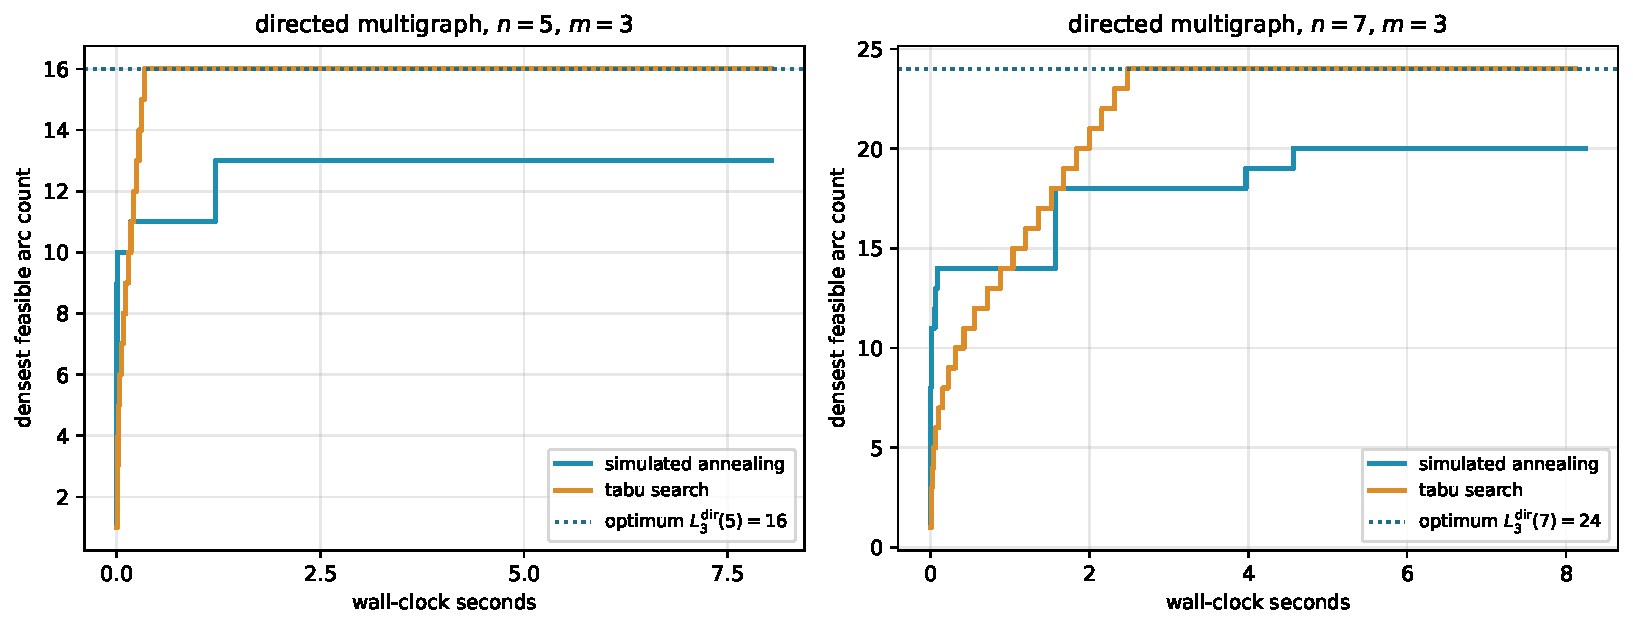
\includegraphics[width=\textwidth]{figures/sa_vs_tabu_convergence.pdf}
    \caption{Densest feasible graph found against wall-clock time, for one simulated-annealing schedule and one tabu schedule on the directed multigraph at $n = 5$ and $n = 7$, $m = 3$. Tabu climbs in a few best-improving steps to the optimum (dotted) and holds, while a single annealing schedule rises quickly and then flattens below it. The time axis is wall-clock on the reference machine, so unlike the seed-reproducible figures elsewhere this one is a representative timed run.}
    \label{fig:sa-vs-tabu}
\end{figure}

This advantage comes at a cost the equal-time comparison already absorbs but is worth naming: each tabu step scans the whole neighbourhood, so it is far more expensive than the annealer's single random proposal, and tabu takes many fewer but better-aimed steps in the same wall-clock. Tabu search is therefore the program's default for solving the problems, reaching every value this thesis reports, the rediscovery of \Cref{tab:rediscovery} and the conjectural lower bounds alike, and reaching the harder directed optima past the exhausted range where the annealer plateaus. Simulated annealing is kept for the self-check and verification, where the small values fall at once, the lighter per-step cost is all that is needed, and its independent restarts parallelise trivially across cores.
\nowreads
The annealer is not the only way to walk this landscape. A natural alternative, suggested by Jan Goedgebeur, is \emph{tabu search} (\Cref{tab:functions} names the implementation), which keeps the energy and the neighbourhood of \Cref{alg:anneal} but replaces the cooling schedule with a deterministic best-improving step. At each step it takes the single-edge move that lowers the energy most, then forbids the pair it just changed for a fixed number of steps, the \emph{tabu tenure}, so the walk cannot immediately undo its last move and stall in a two-step cycle, and when no improving move is left it perturbs the incumbent and carries on. \Cref{tab:sa-vs-tabu} runs the two head to head at an equal budget of six seconds each. On the simple undirected problem both reach the optimum at once. On the two directed problems tabu reaches the target within the budget while the annealer plateaus below it, at sixteen arcs against eighteen and at twenty against the full twenty-four-arc double star, both at $n = 7$. The cause is the one already met at the $n = 8$, $m = 2$ hub stall above: the annealer cools onto whatever dense shape it first reaches and then cannot dismantle it within the budget, whereas tabu's best-improving step follows the steepest density gradient and the tabu list stops it sliding back.

[\dots\ \Cref{tab:sa-vs-tabu} stays here \dots]

Each tabu step scans the whole neighbourhood, so it is far more expensive than the annealer's single random proposal, and takes many fewer but better-aimed steps in the same wall-clock, a cost the equal-time comparison already absorbs. Tabu search is therefore the program's default for solving the problems, reaching every value this thesis reports, the rediscovery of \Cref{tab:rediscovery} and the conjectural lower bounds alike, and reaching the harder directed optima past the exhausted range where the annealer plateaus. Simulated annealing is kept for the self-check and verification, where the small values fall at once, the lighter per-step cost is all that is needed, and its independent restarts parallelise trivially across cores.
\end{offcutrewrite}

\begin{offcutrewrite}{B4. Sections 2.5 and 2.6, pruning and generation}{B4}{chapters/ch2\_certify.tex, the engineering narrative of both sections}{the branch-and-bound figure \textbackslash{}label\{fig:prune\}, and the opening paragraph of the generation section}{Engineering colour only. Every pruning rule, its soundness justification, and the detail establishing complete enumeration were kept: that soundness is what licenses the word \emph{proved}.}
Here \code{solve} changes its implementation without changing its interface. For a simple digraph it runs this branch and bound in place of the blind walk, still with the connectivity checker as the feasibility test, and so reaches the base cases $n \le 7$ that blind enumeration cannot. The booleans alone decide which of the two it uses, and the caller never asks.

Run on the directed $m = 2$ problem \code{solve} returns the complete sequence $2, 4, 6, 8, 10, 12$ for $n = 2, \dots, 7$, each proved complete at its size. The densest digraph it finds at each $n$ is exactly the extremal shape \Cref{ch:basecases} named, the bidirected star (the hub) at every $n < 7$ and, at the crossover $n = 7$ itself, a graph of the tying value $12$ that both the hub and the one-directional bipartite digraph attain. The sweep stops there, so the bipartite side of the crossover is witnessed by the construction and the checker rather than by this search (\Cref{ch:discover} records that the cooled walk in fact stalls on the hub at $n = 8$). Within its range the search therefore confirms not just the values but the winning construction. These are exactly the base cases the induction requires, and with them the long proof of \Cref{thm:dir-arc-m2-exact} rests on a single auditable search rather than on anything done by hand. The exhaustive-search transcript is in \Cref{app:proofs}.

The first way is a search written from scratch. It is a depth-first walk over multiplicity matrices that abandons a branch the moment it turns infeasible or can no longer beat the best graph found, and it keeps just one representative of each isomorphism class by reducing every finished graph to a canonical relabelling, the smallest matrix in dictionary order over all relabellings. The canonical form keeps the memory small, but the time is spent walking labelled partial graphs, and time is what runs out: the full classification at $n = 5$ costs this in-house search about $456$ seconds, and it climbs steeply from there.

The second way (\Cref{tab:functions} names it) does not search at all, it generates, and it was suggested by Prof.\ Jan Goedgebeur. The idea is to hand the hard part, listing one graph per isomorphism class, to a tool that already does it supremely well: the \texttt{geng} program from the \texttt{nauty} toolkit of McKay and Piperno \cite{McKayPiperno14}, invoked through a subprocess and decoded from its \texttt{graph6} output (a compact one-line text encoding of a graph). \texttt{geng} lists the non-isomorphic \emph{undirected} graphs on $n$ vertices, and the program then decorates each one with the directed multiplicities the problem needs, so the isomorphism reduction is inherited for free from the support graph. The decoration itself is plain to state. For one support graph, walk its edges in a fixed order and assign each edge $\{u,v\}$ an ordered pair of multiplicities $\mu(u,v), \mu(v,u)$, each between $0$ and $m-1$ but not both zero, since an edge of the support must carry at least one arc. Along the way the checker measures the partly decorated multigraph, and the moment some pair already exceeds the connectivity ceiling the whole branch of assignments is abandoned, since adding further arcs can never lower a connectivity, the same monotonicity prune as \Cref{fig:prune}. A decoration that survives to the end with the target arc count is kept, reduced to its canonical form so that each isomorphism class is reported once. Different supports share nothing, so they are processed independently across the processor cores. The companion orientation tools \texttt{directg} and \texttt{watercluster2} are not used, because each gives only one orientation per edge and so cannot express the bidirected arcs and repeated multiplicities the extremal graphs are built from. Layering the multiplicities in-house on top of \texttt{geng} is what fits the problem. To be precise about credit: Prof.\ Goedgebeur is not an author of \texttt{nauty}, which is the work of McKay and Piperno cited above. He suggested the generation route, and it is his suggestion that the speed-up rests on.
\nowreads
Run on the directed $m = 2$ problem, with \code{solve} switching to this branch and bound behind an unchanged interface and the booleans alone deciding which engine it uses, the sweep returns the complete sequence $2, 4, 6, 8, 10, 12$ for $n = 2, \dots, 7$, each proved complete at its size. The densest digraph it finds at each $n$ is exactly the extremal shape \Cref{ch:basecases} named, the bidirected star at every $n < 7$ and, at the crossover $n = 7$ itself, a graph of the tying value $12$ that both the hub and the one-directional bipartite digraph attain. The sweep stops there, so the bipartite side of the crossover is witnessed by the construction and the checker rather than by this search (\Cref{ch:discover} records that the cooled walk in fact stalls on the hub at $n = 8$). These are exactly the base cases the induction requires, and with them the long proof of \Cref{thm:dir-arc-m2-exact} rests on a single auditable search rather than on anything done by hand. The transcript is tabulated in \Cref{sec:transcripts}.

[\dots]

The first way is a search written from scratch: a depth-first walk over multiplicity matrices that abandons a branch the moment it turns infeasible or can no longer beat the best graph found, keeping one representative of each isomorphism class by reducing every finished graph to its canonical relabelling, the smallest matrix in dictionary order. The canonical form keeps the memory small, but the time is spent walking labelled partial graphs, and time is what runs out: the full classification at $n = 5$ costs this in-house search about $456$ seconds, and it climbs steeply from there.

The second way (\Cref{tab:functions} names it), suggested by Prof.\ Jan Goedgebeur, does not search at all, it generates. It hands the hard part, listing one graph per isomorphism class, to the \texttt{geng} program of the \texttt{nauty} toolkit of McKay and Piperno \cite{McKayPiperno14}, invoked through a subprocess and decoded from its \texttt{graph6} output. \texttt{geng} lists the non-isomorphic \emph{undirected} graphs on $n$ vertices, and the program decorates each one with the directed multiplicities the problem needs, so the isomorphism reduction is inherited for free from the support graph. The decoration walks the support's edges in a fixed order and gives each edge $\{u,v\}$ an ordered pair of multiplicities $\mu(u,v), \mu(v,u)$, each between $0$ and $m-1$ but not both zero, since an edge of the support must carry at least one arc. The checker measures the partly decorated multigraph as it goes, and the moment some pair exceeds the connectivity ceiling the whole branch of assignments is abandoned, since adding further arcs can never lower a connectivity, the same monotonicity prune as \Cref{fig:prune}. A decoration surviving to the end with the target arc count is kept and reduced to canonical form, so each isomorphism class is reported once, and different supports share nothing, so they are processed independently across the processor cores. The companion orientation tools \texttt{directg} and \texttt{watercluster2} are not used, because each gives only one orientation per edge and so cannot express the bidirected arcs and repeated multiplicities the extremal graphs are built from. To be precise about credit: Prof.\ Goedgebeur is not an author of \texttt{nauty}, which is the work of McKay and Piperno cited above. He suggested the generation route, and it is his suggestion that the speed-up rests on.
\end{offcutrewrite}

\begin{offcutrewrite}{B5. The Contribution Statement}{B5}{main.tex, the objects paragraph and the nine result narratives}{the GenAI disclosure paragraph, ending ``the separate KU Leuven GenAI transparency declaration submitted with the thesis.''}{A second full narrative of every result, which the Short Summary tells and \Cref{ch:synthesis} tells again. Ownership, literature attribution, the credited external suggestion, and the GenAI disclosure are all kept.}
Before listing what is new, it is worth naming the objects, because the results range over a whole family of them and the family is easy to describe. The question never changes. A network is a set of points together with the links between them, two routes through it are \emph{independent} if they share no link, and we ask how many links the network can hold before some pair of points is forced to have $m$ independent routes between them. The number $m$ is a ceiling we impose from outside, so a small $m$ is a strict rule and a large one is lenient. What does change is the kind of network, and it changes along three axes. The first is the model. A \emph{simple graph} allows at most one link between any pair of points, a \emph{multigraph} allows parallel copies of the same link, and an \emph{$r$-uniform hypergraph} replaces the two-endpoint link by a \emph{hyperedge} holding $r$ points at once. The second axis is direction: a link may be two-way, or it may be an \emph{arc} that can be crossed in one direction only. The third is what independence means. Two routes may be asked only to use no common link, which makes them \emph{edge-disjoint}, or they may be asked to avoid one another's interior points as well, which makes them \emph{internally vertex-disjoint} and is the stricter demand. Three models, two directions and two notions of independence give the twelve variants this thesis follows, and the results below are grouped by which of the twelve they concern.

The first concerns hyperedge networks under the stricter notion of independence. At $m=2$ I settle the problem completely for every hyperedge size $r$ and every number of points $n$ (Theorem~\ref{thm:hyper-vertex-m2}). At $m=3$ I prove the matching universal upper bound for $r$-uniform multihypergraphs, and prove that it is attained whenever $r\ge3$ and $2\le\binom{n-2}{r-2}$ (Theorem~\ref{thm:hyper-vertex-m3}). In that range the answer is $\lfloor(m-1)(n-1)/(r-1)\rfloor$, the same number as for the weaker separation, so requiring routes to avoid one another's interiors costs nothing. The $m=3$ upper bound is the harder argument. It rests on a bound for \emph{incidence graphs}, the bipartite graph that records which point lies in which hyperedge, and I prove that bound using Tutte's decomposition of a graph into its three-connected pieces (Lemma~\ref{lem:incidence-rank}).

The second concerns one-way multigraphs, where arcs run in a single direction and may be repeated. Here I prove the exact value, for every $n$ and every $m$ (Theorem~\ref{thm:dir-multi-full}), closing what had stood as a conjecture confirmed only up to six points. The idea is to stop deleting one point at a time. One deletes a whole spanning subgraph instead, chosen sparse and chosen so that it preserves which points can reach which, and such a deletion is guaranteed to lower the number of independent routes for every pair at once, by at least one. Peeling the digraph that way avoids the obstruction that had stopped the point-by-point argument at odd $n$, where the count came out a fraction short, and it needs neither the minimum-degree conjecture the old route leaned on nor any restriction on $m$. One consequence deserves singling out. In three lines it reproves by hand the single finite fact, $L_3^{\mathrm{dir}}(7)=24$, to which the earlier route had reduced the whole $m=3$ problem, and which had been handed to a computation that was abandoned before it ever returned a verdict.

That argument is deliberately blind to which multigraph it takes apart, which is why it had seemed to say nothing about \emph{which} networks actually attain the maximum. Run backwards, from the assumption that its bound is met exactly, it turns out to be rigid. I use that to classify the extremal networks whenever $n \ge \max(8, 2m)$ (Theorem~\ref{thm:dir-multi-uniqueness}), on the branch where the answer grows quadratically in $n$. They are the balanced one-way complete bipartite digraphs at multiplicity $m-1$: split the points into parts whose sizes differ by at most one, choose either part as the source, run an arc from every source point to every point of the other part, and repeat each arc $m-1$ times. For odd $n$, choosing the larger or smaller part as source gives two non-isomorphic reversals. Equality pins the number of strongly connected components, which forces the extremal network to be acyclic, and the triangle-freeness that had served only to keep the deleted subgraph small becomes the equality case of Mantel's theorem, which pins its shape.

The third concerns one-way simple graphs, where each ordered pair of points carries at most one arc. The exact value here is still open for $m \ge 3$, and what I prove is an unconditional bound on it (Proposition~\ref{prop:dir-arc-stability} and Theorem~\ref{thm:dir-arc-linear-error}). Under any route limit $m$, such a graph has at most $\lfloor n^2/4\rfloor + 4(m-1)(n-1)$ arcs. The first term is the size of the one-way bipartite wall, the digraph that splits the points in half and runs every arc from one half to the other, so the bound says that a feasible digraph is within a linear amount of that wall in size. Separately, and this is a claim about shape rather than size, any feasible digraph can be turned into such a wall by deleting at most $\sqrt{m}\,n^{3/2}$ arcs. Together these fix the leading constant of the standing conjecture (Conjecture~\ref{conj:dir-arc}) and the order of its second term, without any assumption about what the extremal graph looks like, which is exactly what every previous route to that bound had needed. What is left is a constant factor of about eight in one coefficient. An external AI review suggested the counting idea behind this estimate. I verified the argument and derived the sharpening stated here.

The fourth concerns multigraphs under the stricter notion of independence, and it needs one sentence of setup. Once routes must avoid one another's interiors, one has to decide whether two parallel copies of the same link count as two independent routes. The convention used through most of this thesis says they do not. Under the other convention, which says they do, the problem is a genuinely different one and is the least understood of the twelve. I settle it at $m=2$, and then disprove the natural guess for larger $m$. The data up to $m=4$ suggest that the best network is a thickened tree, a tree with each of its edges repeated as often as the rule allows. It is not. A bouquet of thickened cliques, all sharing one common point, beats it (Theorem~\ref{thm:clique-chain-vertex}) by a margin that grows linearly in $n$, and its per-vertex rate is quadratic in $m$ rather than linear once $n$ is large enough to pack many blocks (Section~\ref{sec:multi-vertex-standard}). A matching upper bound (Proposition~\ref{prop:multi-vertex-upper}) shows that this is the right joint order in the regime $n/m\to\infty$. Its proof goes through an observation that ties this variant to the oldest one in the family: the underlying simple graph of a feasible multigraph, obtained by forgetting how many copies each link carries, is itself feasible for the simple vertex problem.

Even the bouquet is not the answer, and the next result says what the answer is made of. The value is exactly a \emph{block} problem (Theorem~\ref{thm:multi-vertex-blocks}). A block is a maximal piece of a graph that cannot be broken apart by deleting a single one of its points. The objective turns out to be a sum of local terms, one for each edge of the underlying simple graph, and no route between two adjacent points ever leaves the block those two share, so the total is additive over blocks. The whole question then reduces to a knapsack: decide how to divide the points into blocks, and use the best two-connected block of each size. That settles the value exactly for every $n \le 8$ and $m \le 8$, and it shows the bouquet is the wrong shape. Within those enumerated cases, whenever $m\ge5$ a single block spanning all the points beats every way of splitting them. The blocks that win are bipartite rather than complete, and thickening those instead (Theorem~\ref{thm:multi-vertex-bipartite}) improves the constant by a factor $8(3-2\sqrt2) \approx 1.373$, closing part of the gap to the upper bound.

Two further results come from asking what the quadratic bound above actually uses. The answer is very little: one cap on one family of routes, and after that nothing but counting degrees (Lemma~\ref{lem:two-step-budget}). Stated that way the argument reaches well beyond the case it was proved for, since any variant able to supply the cap inherits the bound. These results reuse the externally suggested counting idea credited above, and my contribution here is the weaker hypothesis and the two arguments that supply it. The multigraph upper bound just mentioned is not one of the two, and reaches its conclusion by an unrelated route through Mader's density theorem.

The first of the two returns to one-way simple graphs, now under the stricter notion of independence. The thesis is otherwise careful to keep that problem apart from the arc one, because Whitney's inequality between the two runs the wrong way and an upper bound on the arc problem says nothing about this one. Here the transfer is legitimate, because what carries across is the family of routes the argument counts and not the bound itself. For every fixed $m\ge3$ the result is $k_m^{\mathrm{dir}}(n) = n^2/4 + \Theta_m(n)$ (Theorem~\ref{thm:dir-vertex-linear-error}), and at $m=2$ the exact theorem gives $n^2/4+O(1)$. Thus the leading constant is settled on this side too and the two one-way problems agree to first order.

The second settles the leading constant for one-way hyperedge networks outright (Theorem~\ref{thm:dir-hyper-constant}). The maximum is $(1+o(1))(m-1)n^2/\bigl(4(r-1)\bigr)$ for every fixed $r$ and $m$, and under both notions of independence at once, so the bipartite construction is asymptotically optimal and the factor of four that had separated the known bounds is closed. The obstacle here was a real one. A hyperedge carries $r-1$ heads at a time, so two routes leaving the same point through different hyperedges need not be independent at all. The argument does not repair that. It pays the factor $r-1$, then shows the payment lands in the linear error term rather than in the leading one, while a second factor of $r-1$, arriving from somewhere else entirely, divides the leading term.

That proof reads a one-way hyperedge as a single tail fanning out to many heads. The last result is that the same leading constant holds for every other way of orienting a hyperedge, that is, for any split of its $r$ points into tails and heads (Theorem~\ref{thm:dir-hyper-general-constant}). The single tail had been doing double duty, once for the routes entering a hyperedge and once for those leaving it, and with several tails the two sides interfere. The repair is to stop building a large family of routes and instead take a maximum family and read off what stopped it, since every route left out is blocked by a hyperedge that family has already used, and a hyperedge has only $r$ points to block with. So the orientation axis closes to first order: forward, backward and every mixture between them share the same leading term.
\nowreads
What is new in this thesis is told in full in \Cref{ch:synthesis} and proved in \Cref{app:proofs}. Listed compactly, and grouped by which of the twelve variants each concerns, my own results are these.

\begin{itemize}
  \item \emph{Hyperedge networks, vertex separation.} The problem is settled completely at $m = 2$, for every hyperedge size $r$ and every $n$ (\Cref{thm:hyper-vertex-m2}). At $m = 3$ I prove the universal upper bound $\floor{(m-1)(n-1)/(r-1)}$ for $r$-uniform multihypergraphs and prove it attained whenever $r \ge 3$ and $2 \le \binom{n-2}{r-2}$ (\Cref{thm:hyper-vertex-m3}), so in that range requiring routes to avoid one another's interiors costs nothing. The upper bound is the harder argument and rests on a new rank bound for incidence graphs, proved by way of Tutte's decomposition into three-connected pieces (\Cref{lem:incidence-rank}).

  \item \emph{One-way multigraphs.} The exact value, for every $n$ and every $m$ (\Cref{thm:dir-multi-full}), closing what had stood as a conjecture confirmed only to six vertices. The idea is to delete a whole sparse spanning subgraph chosen to preserve reachability, rather than one vertex at a time, which avoids the obstruction that stopped the point-by-point argument at odd $n$ and needs no restriction on $m$. In three lines it also reproves by hand the finite fact $L_3^{\mathrm{dir}}(7) = 24$, to which the earlier route had reduced the whole $m = 3$ problem. Read backwards from equality the same argument is rigid, and classifies the extremal digraphs on the quadratic branch whenever $n \ge \max(8, 2m)$ as the balanced one-way complete bipartite digraphs at multiplicity $m-1$ (\Cref{thm:dir-multi-uniqueness}).

  \item \emph{One-way simple graphs, arc separation.} The exact value is open for $m \ge 3$; what I prove is an unconditional bound on it, $\floor{n^2/4} + 4(m-1)(n-1)$ arcs under any route limit $m$ (\Cref{prop:dir-arc-stability,thm:dir-arc-linear-error}). Together these fix the leading constant of the standing conjecture (\Cref{conj:dir-arc}) and the order of its second term with no assumption about the shape of the extremiser, which is exactly what every previous route to that bound had needed. Separately, and this is a claim about shape rather than size, any feasible digraph becomes a one-way bipartite wall after deleting at most $\sqrt{m}\,n^{3/2}$ arcs. An external AI review suggested the counting idea behind this estimate. I verified the argument and derived the sharpening stated here.

  \item \emph{Multigraphs, vertex separation, counting parallel copies as distinct routes.} This is the least understood of the twelve. I settle it at $m = 2$, then disprove the natural guess: the thickened tree the data up to $m = 4$ suggest is beaten, for every $m \ge 5$, by a bouquet of thickened cliques sharing one point, by a margin growing linearly in $n$ (\Cref{thm:clique-chain-vertex}), and a matching upper bound gives the right joint order in the regime $n/m \to \infty$ (\Cref{prop:multi-vertex-upper}). Even the bouquet is not the answer: the value is exactly a \emph{block} problem, a knapsack over the best two-connected block of each size (\Cref{thm:multi-vertex-blocks}), which settles it for every $n \le 8$ and $m \le 8$ and shows the winning blocks are bipartite rather than complete (\Cref{thm:multi-vertex-bipartite}).

  \item \emph{Two results from isolating what the quadratic bound uses.} The answer is very little: one cap on one family of routes, and after that nothing but counting degrees (\Cref{lem:two-step-budget}), so any variant able to supply the cap inherits the bound. Hence $k_m^{\mathrm{dir}}(n) = n^2/4 + \Theta_m(n)$ for every fixed $m \ge 3$ (\Cref{thm:dir-vertex-linear-error}), a legitimate transfer because what carries across is the family of routes counted and not the bound itself, Whitney's inequality running the wrong way for the latter. And the leading constant for one-way hyperedge networks is settled outright at $(m-1)n^2/\bigl(4(r-1)\bigr)$, under both separations at once (\Cref{thm:dir-hyper-constant}), then extended to every way of splitting a hyperedge into tails and heads (\Cref{thm:dir-hyper-general-constant}), so the orientation axis closes to first order. These two reuse the externally suggested counting idea credited above, and my contribution here is the weaker hypothesis and the two arguments that supply it. The multigraph upper bound just mentioned is not one of them, and reaches its conclusion by an unrelated route through Mader's density theorem.
\end{itemize}
\end{offcutrewrite}

\begin{offcutrewrite}{B5 (continued). The three jobs paragraph}{B5}{main.tex, Contribution Statement}{the ownership paragraph, ending ``do not depend on their splitting-off theorem.''}{The measure/prove/discover split is stated in the Foreword and argued in \Cref{ch:certify}. The honesty contract at the end of it is kept.}
The program has three jobs, and it keeps them separate. It \emph{measures}: given any graph, it computes exactly, through maximum flow, how many independent routes the busiest pair of vertices has. It \emph{proves}: for a fixed number of vertices it sweeps a finite space of graphs, and when nothing in that space beats a target, that sweep is a genuine upper-bound proof for that finite space. And it \emph{discovers}: a search guided by metaheuristics wanders the space of graphs and finds dense ones, which give lower bounds and suggest conjectures but never prove an upper bound by themselves. Every general statement in the thesis rests on a proof by hand or a cited theorem. The computer searches are evidence that points the way, never a replacement for the argument.
\nowreads
The program has three jobs and keeps them separate: it \emph{measures} connectivity exactly by maximum flow, it \emph{proves} a finite optimum by sweeping a finite space of graphs, and it \emph{discovers} dense graphs by metaheuristic search, which gives lower bounds and suggests conjectures but never an upper bound. Every general statement in the thesis rests on a proof by hand or a cited theorem. The computer searches are evidence that points the way, never a replacement for the argument.
\end{offcutrewrite}

\begin{offcutrewrite}{B6. Appendix A.1, Menger and Gomory--Hu}{B6}{chapters/app\_proofs.tex, the scope discussion and the existence sketch}{the statement of \Cref{thm:menger}, and the paragraph on the symmetry requirement}{Proof sketches shortened. Precise statements, citations, the symmetry caveat, and \Cref{lem:degree-bound} in full are all kept, as is A.2, Mader in full.}
A directed capacitated graph is the most general object here, and every graph model the thesis uses is a special case of it. An undirected graph is the symmetric case, each edge a pair of opposite unit-capacity arcs. A multigraph is the integer-capacity case, with $\mu(u,v)$ units on the pair $uv$. The hypergraph version (\Cref{thm:menger-hyper}) is this very theorem applied to the helper-point network of \Cref{fig:hyper-gadget}, a capacitated digraph. The \emph{internally vertex-disjoint} version is obtained not by changing the theorem but by changing the graph it runs on, a device called \emph{vertex splitting}: replace each internal vertex $w$ by two copies joined by a single unit-capacity arc $w^- \to w^+$, send every arc that entered $w$ into $w^-$ and every arc that left $w$ out of $w^+$. A flow may now pass through $w$ at most once, so edge-disjoint paths in the split graph are exactly internally vertex-disjoint paths in the original, and a minimum edge cut there is a minimum vertex cut here. This split graph is literally what the checker of \Cref{ch:certify} builds, which is why a single maximum-flow routine measures all four separations.

Existence rests on a single property of cuts. Write $d(S)$ for the capacity of the cut $(S, V \setminus S)$. This function is \emph{submodular}, meaning that $d(A) + d(B) \ge d(A \cap B) + d(A \cup B)$ for any two vertex sets $A$ and $B$. That is exactly the inequality which lets a cheapest $u$--$v$ cut crossing some other set $S$ be traded for one that does not, without ever losing capacity. Building the tree is then $n-1$ rounds of one minimum-cut computation each, each round splitting one bag of the current tree along a fresh minimum cut, with that trading property (the \emph{uncrossing} lemma) guaranteeing no earlier round's cut is ever spoiled by a later one. The full construction, uncrossing induction included, is in Gomory and Hu's original paper \cite{GomoryHu61}.
\nowreads
Every graph model the thesis uses is a special case of a directed capacitated graph: an undirected graph is the symmetric one, each edge a pair of opposite unit-capacity arcs; a multigraph is the integer-capacity one, with $\mu(u,v)$ units on the pair $uv$; and the hypergraph version (\Cref{thm:menger-hyper}) is this very theorem applied to the helper-point network of \Cref{fig:hyper-gadget}. The \emph{internally vertex-disjoint} version is obtained not by changing the theorem but by changing the graph it runs on, a device called \emph{vertex splitting}: replace each internal vertex $w$ by two copies joined by a single unit-capacity arc $w^- \to w^+$, send every arc that entered $w$ into $w^-$ and every arc that left $w$ out of $w^+$. A flow may then pass through $w$ at most once, so edge-disjoint paths in the split graph are exactly internally vertex-disjoint paths in the original, and a minimum edge cut there is a minimum vertex cut here. This split graph is what the checker of \Cref{ch:certify} builds, which is why a single maximum-flow routine measures all four separations.

[\dots]

Existence rests on a single property of cuts. Writing $d(S)$ for the capacity of the cut $(S, V \setminus S)$, this function is \emph{submodular}: $d(A) + d(B) \ge d(A \cap B) + d(A \cup B)$ for any two vertex sets. That is exactly the inequality which lets a cheapest $u$--$v$ cut crossing some other set be traded for one that does not, without losing capacity, and the tree is then built in $n-1$ rounds of one minimum-cut computation each, that trading property (the \emph{uncrossing} lemma) guaranteeing no earlier round's cut is spoiled by a later one. The construction, uncrossing induction included, is in Gomory and Hu's original paper \cite{GomoryHu61}.
\end{offcutrewrite}

\begin{offcut}{B7. Five thin wrapper codecards}{B7}{chapters/ch2\_certify.tex and chapters/ch3\_discover.tex}{each card sat directly after the paragraph that explains what it wraps; their content is now in \Cref{app:software-map}}{Ten cards were more than the argument needed. Five central ones stay, beside \code{solve}, the model, the checker, the prover, and the search, so the measure-prove-discover split is still visible where it is argued.}
\codecard{local\_edge\_connectivity(G, s, t) $\to \mathbb{N}$}{MEASURE}
{a graph $G$ and an ordered pair $(s,t)$}
{$\lambda_G(s,t)$, the maximum number of edge-disjoint $s$--$t$ paths}
{a single \code{scipy.sparse.csgraph.maximum\_flow} on the network whose arc capacities are the multiplicities $\mu$, so by Menger the flow value is the path count.}

\codecard{max\_vertex\_connectivity(G) $\to \mathbb{N}$}{MEASURE}
{a graph $G$}
{$\kappa^{\max}(G)$, the largest local vertex-connectivity over all pairs}
{the same sweep as the edge checker, but each flow runs on the split capacity matrix \code{\_split\_capacity\_matrix(G)} of \Cref{fig:vertex-split}, so the unit internal arcs count internally vertex-disjoint paths. Parallel edges are given capacity one here, so they never raise $\kappa$.}

\codecard{max\_edge\_connectivity\_via\_tree(G) $\to \mathbb{N}$}{MEASURE}
{an undirected graph $G$}
{$\lambda^{\max}(G)$, identical to the pairwise sweep}
{build one Gomory--Hu tree with \code{networkx.gomory\_hu\_tree}, then return its heaviest edge, which costs $n-1$ flows in place of $\binom{n}{2}$ and cross-checks the checker.}

\codecard{max\_hyperedge\_connectivity(H) $\to \mathbb{N}$}{MEASURE}
{an $r$-uniform hypergraph $H$}
{$\lambda^{\max}(H)$, the largest Berge edge-connectivity over all pairs}
{build the enlarged capacity matrix \code{\_hyper\_capacity\_matrix(H)} in which every hyperedge becomes a helper point that only one route may pass through, then take the same maximum flow as the graph checker. On two-vertex hyperedges it matches ordinary edge-connectivity.}

\codecard{edge\_sensitivity(G, u, v) $\to \mathbb{N}$}{MEASURE}
{a graph $G$ and one of its edges $e = (u,v)$}
{$\sigma(e) = \lambda^{\max}(G) - \lambda^{\max}(G - e)$}
{delete $e$ and let the checker remeasure, where a positive value marks a load-bearing edge. The whole-graph version \code{sensitivity\_map(G)} reuses one shared baseline measurement. This single number is the dial the cooling turns.}
\end{offcut}

\section*{Group C: structural}
\addcontentsline{toc}{chapter}{Group C: structural}
\markboth{Group C: structural}{Group C: structural}

\begin{offcutrewrite}{C1. The twelve-variant sweep, narrated twice}{C1}{chapters/ch3\_discover.tex, the three-regimes walk in the trichotomy section}{the two features of the directed-arc panels, ending ``one that survives the case that broke the previous guess.''}{Chapter 3 keeps the trichotomy definition and one worked case, the directed simple arc problem where the proved-to-conjectured boundary is sharp. \Cref{ch:synthesis} keeps the authoritative table, the tree, and the qualifications. The Whitney caution was kept in Chapter 3, since it is about what the program had to compute.}
Asking the same three questions of every variant, the answers sort into three regimes, and \Cref{fig:variant-bounds-m3} shows all twelve at once, one panel per variant, in exactly this proved, conjectured, and guessed language.

In the first regime the closed form is already a theorem throughout the stated model and parameter range, proved by hand in \Cref{ch:basecases} or cited, and the computation only confirms it. Several families live here. The simple-graph and multigraph undirected edge families do for every $m$, and the hypergraph edge family joins them in the attainment ranges of \Cref{prop:hyper-edge,thm:simple-hyper-edge}. The directed problems at $m = 2$ and the directed multigraph arc problem at every $m$ also belong here (\Cref{thm:dir-multi-full}). So do the undirected vertex families, but only in ranges that differ by model: through $m \le 4$ for simple graphs and multigraphs (\Cref{thm:leonard}), while for hypergraphs $m=2$ is unconditional and the exact $m=3$ value is proved when $r\ge3$ and $2\le\binom{n-2}{r-2}$ (\Cref{thm:hyper-vertex-m2,thm:hyper-vertex-m3}). Outside those ranges the same rows drop into the third regime below, which is why the leaf colours of \Cref{fig:variant-tree-status} are stated at general $m$ and \Cref{tab:summary} carries the exact conditions. For these the certified small cases and the rediscovered constructions of \Cref{tab:rediscovery} are validation, not new knowledge: the formula was never in doubt, and the program's role is to check that the pipeline reproduces it. That the two multigraph vertex rows measure exactly as their underlying simple graphs is a matter of the counting convention of \Cref{sec:parallel-convention} rather than a theorem, so those rows need no computation of their own at all.

The directed vertex rows do need their own computation. Whitney's inequality $\kappa^{\max} \le \lambda^{\max}$ means every graph feasible for the arc problem is automatically feasible for the vertex problem too, since a small $\lambda^{\max}$ forces an even smaller $\kappa^{\max}$. So the arc problem's own dense construction doubles as a valid witness, hence a lower bound, for the vertex problem. But it supplies no upper bound: a bound proved only for the smaller arc-feasible family says nothing about the larger vertex-feasible family, which may contain denser graphs the arc argument never had to rule out. So they get their own: every exact point on those panels comes from the search and the exhaustion run under the vertex test.

In the second regime the three columns genuinely differ and the computation is load-bearing. This is the regime of the worked example above. The directed simple arc and vertex problems at $m \ge 3$ are proved only at the small $n$ the exhaustion reaches and conjectured by the search beyond, with the formula of \Cref{conj:dir-arc} the through-line.

The directed multigraph arc problem used to sit here and no longer does. It has moved up into the first regime, since \Cref{thm:dir-multi-full} proves $L_m^{\mathrm{dir}}(n) = (m-1)\max(2(n-1), \floor{n^2/4})$ for every $n$ and every $m$, with no parity split and no auxiliary conjecture. Its panel is worth watching all the same, because it is the one place in the grid where the computation and the proof were developed against each other rather than in sequence. In its cut-counting mode \code{solve} proves the $m$-free number $M^{*}(n) = 2(n-1)$ outright for $n \le 6$. The scaling identity $L_m^{\mathrm{dir}}(n) = (m-1)\,M^{*}(n)$ of \Cref{ch:certify} then carries that one certified number to every $m$ at once. Those certificates were the evidence that the closed form was right long before the proof of it existed, and they now serve as an independent check on a theorem rather than as the reason to believe a conjecture.

In every row of this regime the formula agrees with proof where proof reaches and with the search where it does not, exactly the linkage the worked example displayed.

In the third regime there is no formula at all, and the honesty is in drawing the guess as a guess. The undirected vertex problem at $m \ge 6$ has been open since 1974 with its extremal structure genuinely unknown. The undirected hypergraph vertex problem joins it at $m\ge4$, and the small parameter range not covered by the $m=3$ attainment theorem remains outside the proved curve as well. At $m=2$ its value is settled for every uniformity and every $n$, and at $m=3$ the exact value is proved when $r\ge3$ and $2\le\binom{n-2}{r-2}$ (\Cref{thm:hyper-vertex-m2,thm:hyper-vertex-m3}). The two \emph{directed} hypergraph variants are in the third regime at every $m$, and they need a one-tail, many-head reading of a Berge edge that this thesis defines itself only so that \code{solve} can measure it at all. Here the program still computes exact values at the few sizes that finish, and its search still exhibits feasible graphs at a handful more, but no closed form is in sight. What is known there is asymptotic rather than exact: \Cref{thm:dir-hyper-constant} pins the leading term at $(m-1)n^2/(4(r-1))$ for both separations, which is a statement about where these curves are heading and not one a panel at $n \le 10$ can display. The panels carry a yellow line that simply interpolates the machine points in straight segments, trusted no further than the eye. We draw it \emph{through} the points rather than fitting a smooth curve above them: the points are honest lower bounds, the truth lies on or above them, and a line riding above the points would claim more than the search ever found.
\nowreads
Asking the same three questions of every variant sorts the twelve into three regimes: those where the closed form is already a theorem and the computation only confirms it, those where proof reaches the small sizes and the search carries the rest with one formula threading through both, and those where there is no formula at all and the honesty lies in drawing the guess as a guess. \Cref{fig:variant-bounds-m3} shows all twelve at once in exactly that proved, conjectured, and guessed language, and \Cref{ch:synthesis} places every variant in its regime with the exact conditions attached (\Cref{tab:summary} and \Cref{fig:variant-tree-status}).

One qualification belongs here rather than there, because it is about what the program had to compute. On the two directed \emph{vertex} panels every exact point comes from the exhaustion and the search re-run under the vertex test, not inherited from the arc runs. Whitney's inequality $\kappa^{\max} \le \lambda^{\max}$ makes every arc-feasible graph vertex-feasible, so an arc construction is a legitimate witness and hence a lower bound there. It supplies no upper bound: a ceiling proved only for the smaller arc-feasible family says nothing about the larger vertex-feasible one, which may contain denser graphs the arc argument never had to rule out.
\end{offcutrewrite}

\begin{offcut}{C3. The Chernoff primer}{C3}{chapters/app\_proofs.tex, appendix A.10}{the sentence ``The probabilistic ingredients are two Chernoff bounds, quoted in the form we use them.''}{Textbook intuition for a bound the thesis only quotes. \Cref{thm:chernoff}, \Cref{cor:chernoff-degree}, and the two-case proof of \Cref{thm:gnp-threshold} all stay.}
\begin{primer}[Primer: what a Chernoff bound says]
Both proofs below need to say that a sum of many independent yes-or-no trials
almost never lands far from its average. That is the content of a \emph{Chernoff
bound}, and the intuition is worth stating even though we only quote the result.
Let $X = X_1 + \dots + X_N$ count the successes among independent trials, with mean
$\mu = \mathbb{E}[X]$. A Chernoff bound says the chance that $X$ overshoots $\mu$ by
a factor $1 + \delta$, or undershoots it by a factor $1 - \delta$, decays
\emph{exponentially} in $\mu$, not merely polynomially as Chebyshev's inequality
would give. The mechanism is a single trick. Rather than bound $\Pr[X \ge a]$
directly, bound $\Pr[e^{tX} \ge e^{ta}]$ by Markov's inequality for a parameter
$t > 0$, use independence to factor $\mathbb{E}[e^{tX}] = \prod_i \mathbb{E}[e^{t
X_i}]$ into a product over the trials, and then choose $t$ to make the resulting
bound as small as possible. The exponential in the answer is exactly the $e^{tX}$
that was fed through Markov. We quote the two tails in the shape the threshold
proof consumes.
\end{primer}
\end{offcut}

\begin{offcutrewrite}{C3 (continued). The random-graph prose in Chapter 1}{C3}{chapters/ch1\_basecases.tex, the setup paragraphs and one overclaim}{the opening of the random-graphs section, and the paragraph on why the two connectivities pull apart}{Two setup paragraphs merged. Separately, the closing claim read the sampling figure as evidence for the $m=5$ extremal divergence, which it does not show: it shows the two notions coming apart on a fraction of random samples, which is a real but different observation. \Cref{fig:edge-vertex} itself stays and its caption was already correct.}
The random model is the natural place to build intuition, because it shows the qualitative behaviour of the connectivity notions before any construction is pushed to its limit, and we will return to it whenever a picture of the typical graph clarifies a result. It is not a detour from the program to come, either: a sampled $G(n,p)$ is an ordinary graph, measured by the very same connectivity checker the next chapter builds for every other variant, so the random model is simply the one pipeline turned to \emph{observe} the typical case rather than to prove or to discover the extremal one.

Each of the $\binom{n}{2}$ possible edges of $G(n, p)$ is included independently with probability $p$, and on the resulting graph we read off both binding connectivities, the edge version $\lec_G^{\max}$ and the vertex version $\kap_G^{\max}$, from the very same sample. Whitney's inequality $\kap_G^{\max} \le \lec_G^{\max}$ guarantees the vertex value never exceeds the edge one, but it is silent on how often the two actually come apart.

In the dense limit the graph approaches the complete graph, where $\kap^{\max} = \lec^{\max} = n - 1$ for every pair and the gap closes entirely. The divergence the thesis records at $m = 5$ is therefore not an artefact of the extremal construction. It is already there, in miniature, in the random model.
\nowreads
The random model is the natural place to build intuition, because it shows the qualitative behaviour of the connectivity notions before any construction is pushed to its limit. It is not a detour from the program to come, either: a sampled $G(n,p)$ is an ordinary graph, measured by the very same connectivity checker the next chapter builds for every other variant. Each of the $\binom{n}{2}$ possible edges of $G(n,p)$ is included independently with probability $p$, and on the resulting graph we read off both binding connectivities from the same sample. Whitney's inequality $\kap_G^{\max} \le \lec_G^{\max}$ guarantees the vertex value never exceeds the edge one, but it is silent on how often the two actually come apart.

[\dots]

In the dense limit the graph approaches the complete graph, where $\kap^{\max} = \lec^{\max} = n - 1$ for every pair and the gap closes entirely. What this shows is not the $m = 5$ extremal divergence, which is a statement about the densest graphs the ceiling allows and not about typical ones. It is the separate and weaker fact that the two notions do come apart in ordinary graphs, and that they do so exactly where routes are forced through a shared bottleneck vertex, which is the mechanism the extremal constructions go on to exploit deliberately.
\end{offcutrewrite}


\end{document}
